%%____________________________________________________________________________||
\section{Physics performance}
\label{sec:physics}

%%____________________________________________________________________________||
\subsection{Key distributions for the hadronic signal
  region\label{sec:mc-data-comp}}

%Distributions of key analysis variables 
The hadronic signal region selection is detailed in Sec.~\ref{sec:hadSelection}.

PLACEHOLDER: plots of alphaT for signal region, HT, MHT, njet

%%____________________________________________________________________________||
\subsection{Breakdown of SM backgrounds in the hadronic signal
  region\label{sec:bkgd-comp}}

In the absence of multijet events from QCD, the remaining significant
backgrounds in the signal region are expected to stem from SM
processes with genuine \met in the final state. For the low jet
multiplicity categories, the largest backgrounds with genuine \met are
generally from the associated production of W or Z bosons with jets,
followed by either the weak decays \znunu\ or \wtaunu, where the
$\tau$ decays hadronically and is identified as a jet, or by leptonic
decays that are outside acceptance or not rejected by the dedicated
electron or muon vetoes. For the higher jet multiplicity categories,
top quark production followed by semileptonic weak top quark decay
becomes important. The relative contribution from \ttbar is enhanced
or suppressed depending on the number of b-jets required. 
% A breakdown
% of the relative contributions of the SM backgrounds, as given by
% simulation, in the different (\njet, \nb, \scalht) bins can be found
% in Table~\ref{tab:backgrounds}. 
A plot showing the yields for these electroweak backgrounds and a reference
signal model can be seen in Figs~\ref{fig:ewkYields1}-\ref{fig:ewkYields4}. 
A breakdown of the three
dominant channels, \zInv , \ttbar and W~+~jets, are shown. The contribution from
other sources, such as the single top and diboson channels, was found to be
negligible so are not shown.

\begin{figure}[]
  \centering
  \subfigure[Hadronic signal region yields for electroweak backgrounds
  ($\njet = 2$)]{
    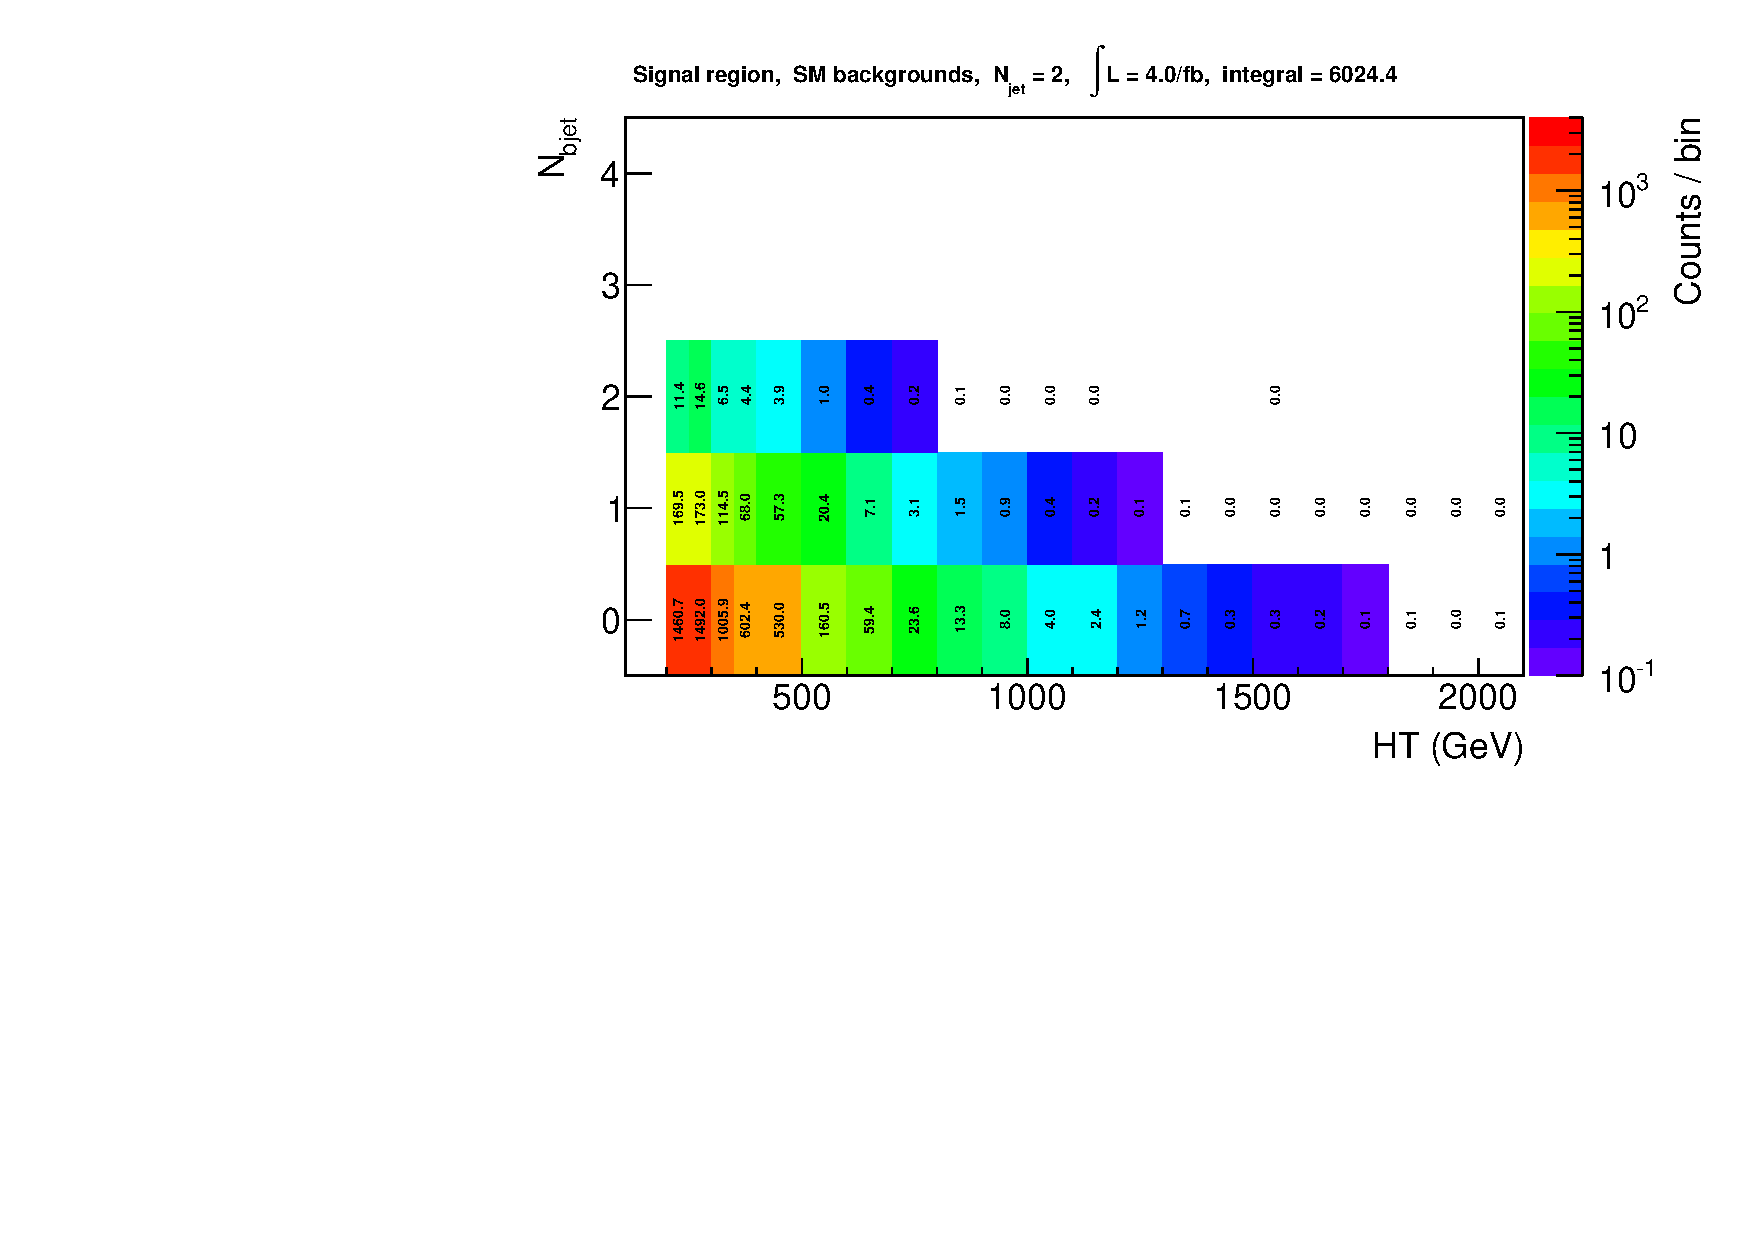
\includegraphics[width=0.5\textwidth]{figures/yieldPlots/had_ewk_eq2j.pdf}
  }~~
  \subfigure[Hadronic signal region yields for the \zInv background
  ($\njet = 2$)]{
    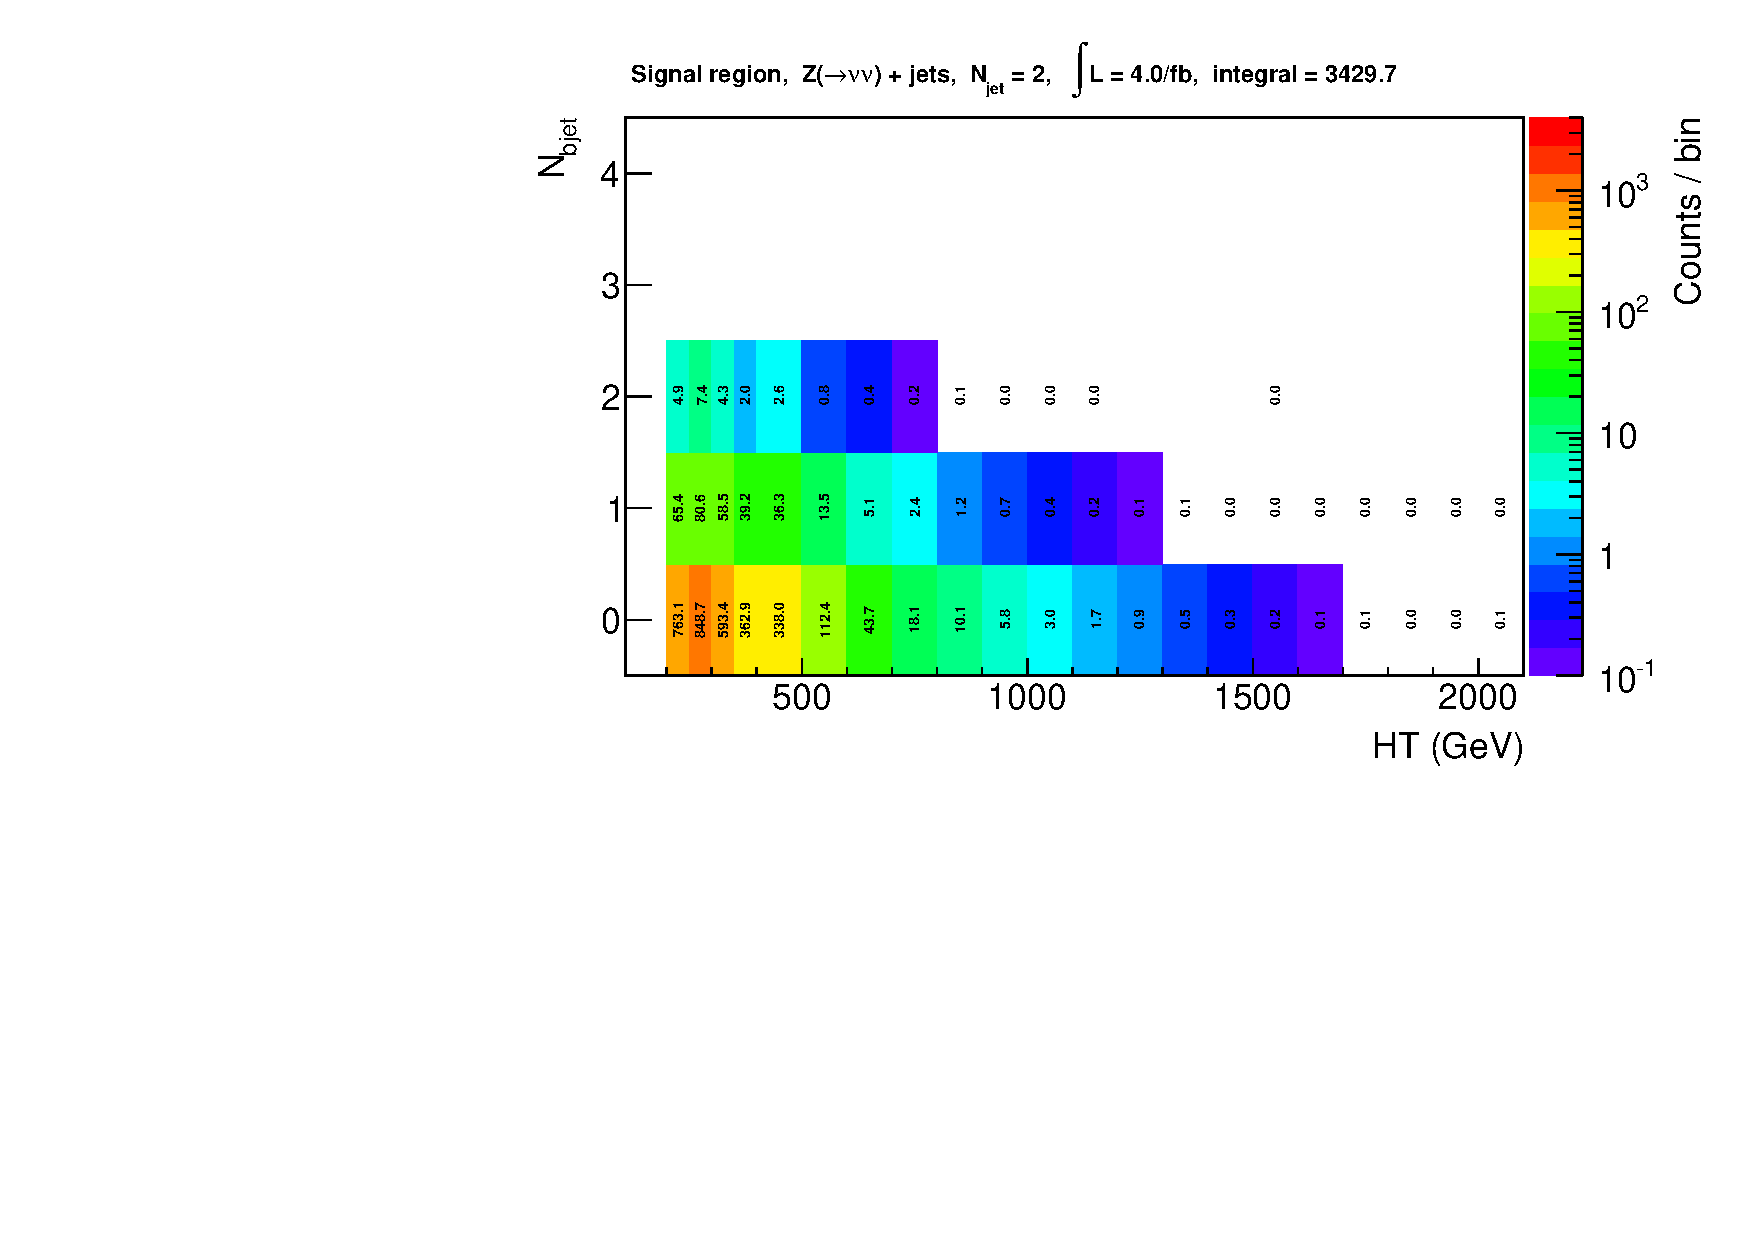
\includegraphics[width=0.5\textwidth]{figures/yieldPlots/had_zinv_eq2j.pdf}
  }\\
  \subfigure[Hadronic signal region yields for W~+~jets backtround
  ($\njet = 2$)]{
    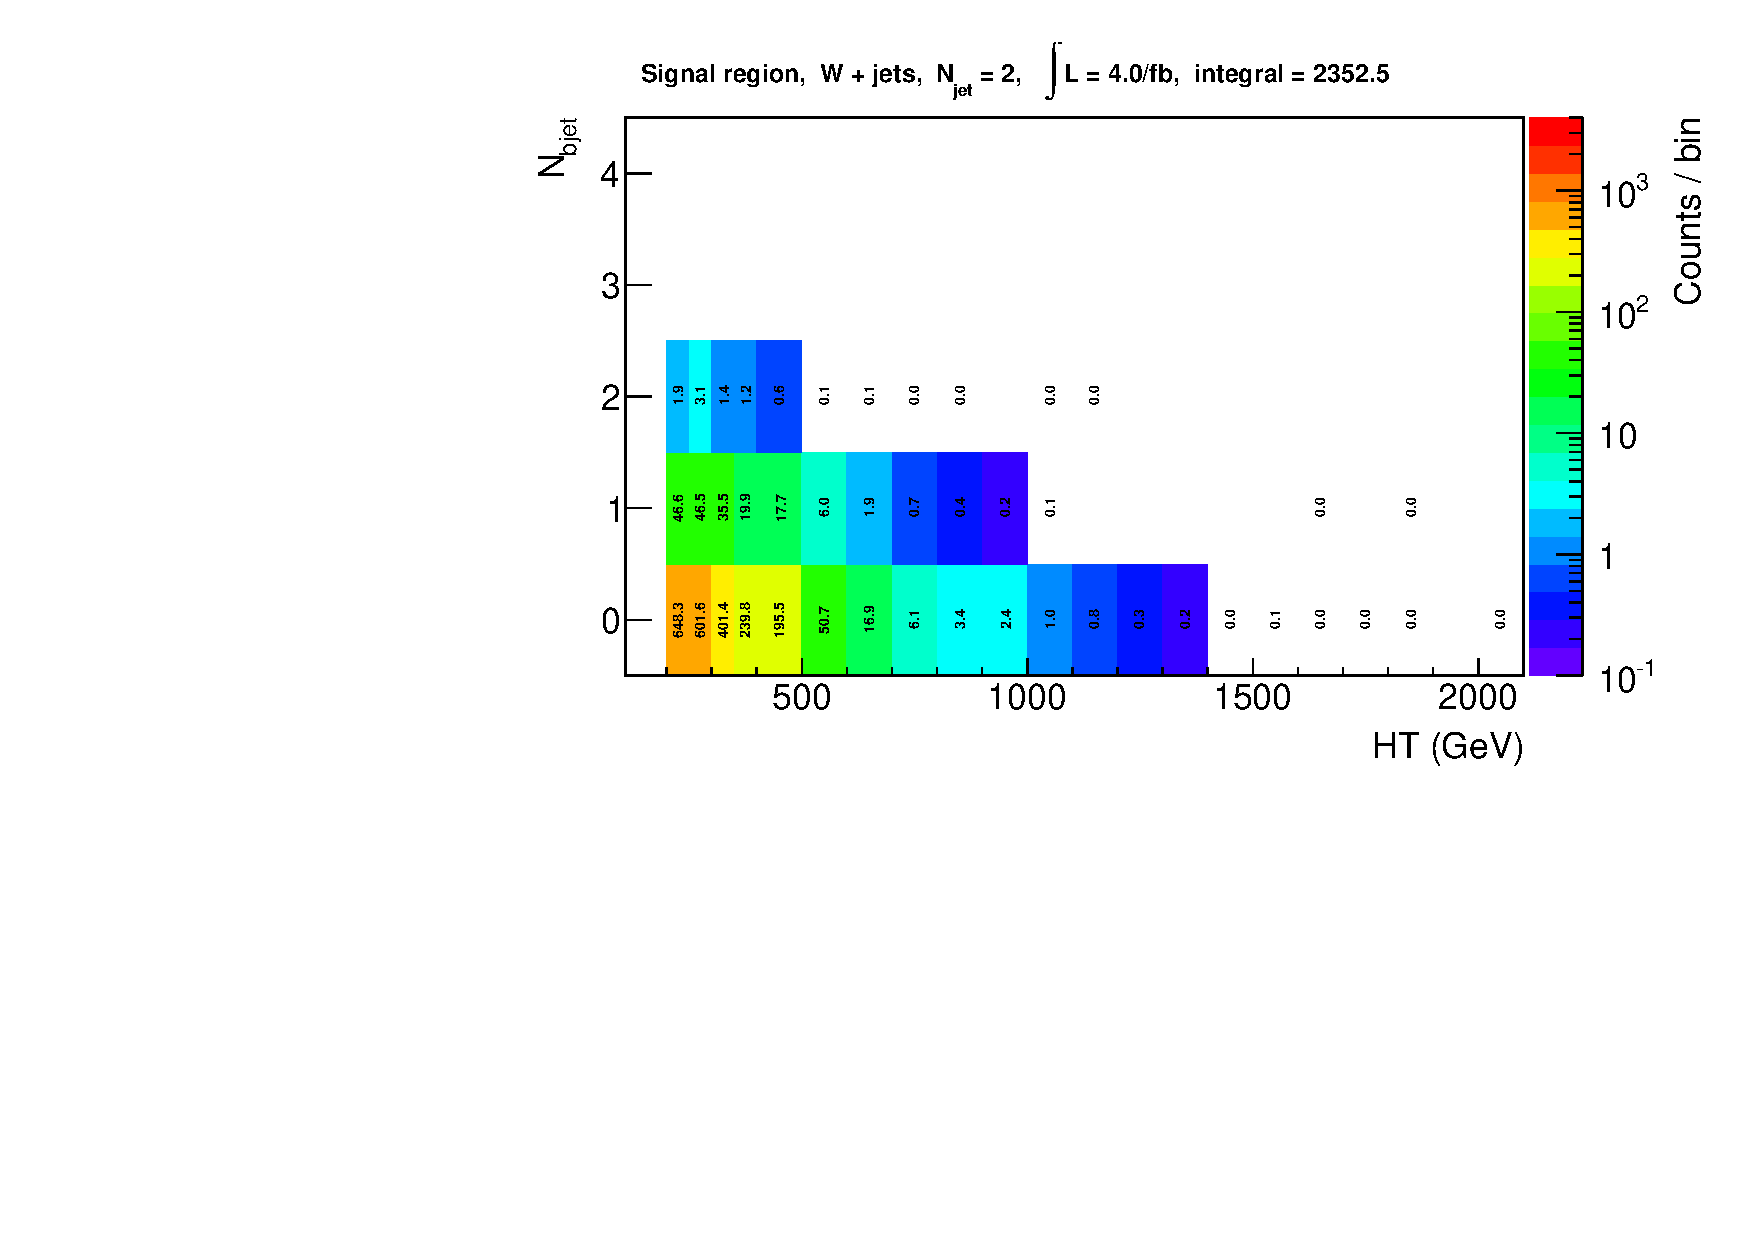
\includegraphics[width=0.5\textwidth]{figures/yieldPlots/had_wjets_eq2j.pdf}
  }~~
  \subfigure[Hadronic signal region yields for \ttbar background
  ($\njet = 2$)]{
    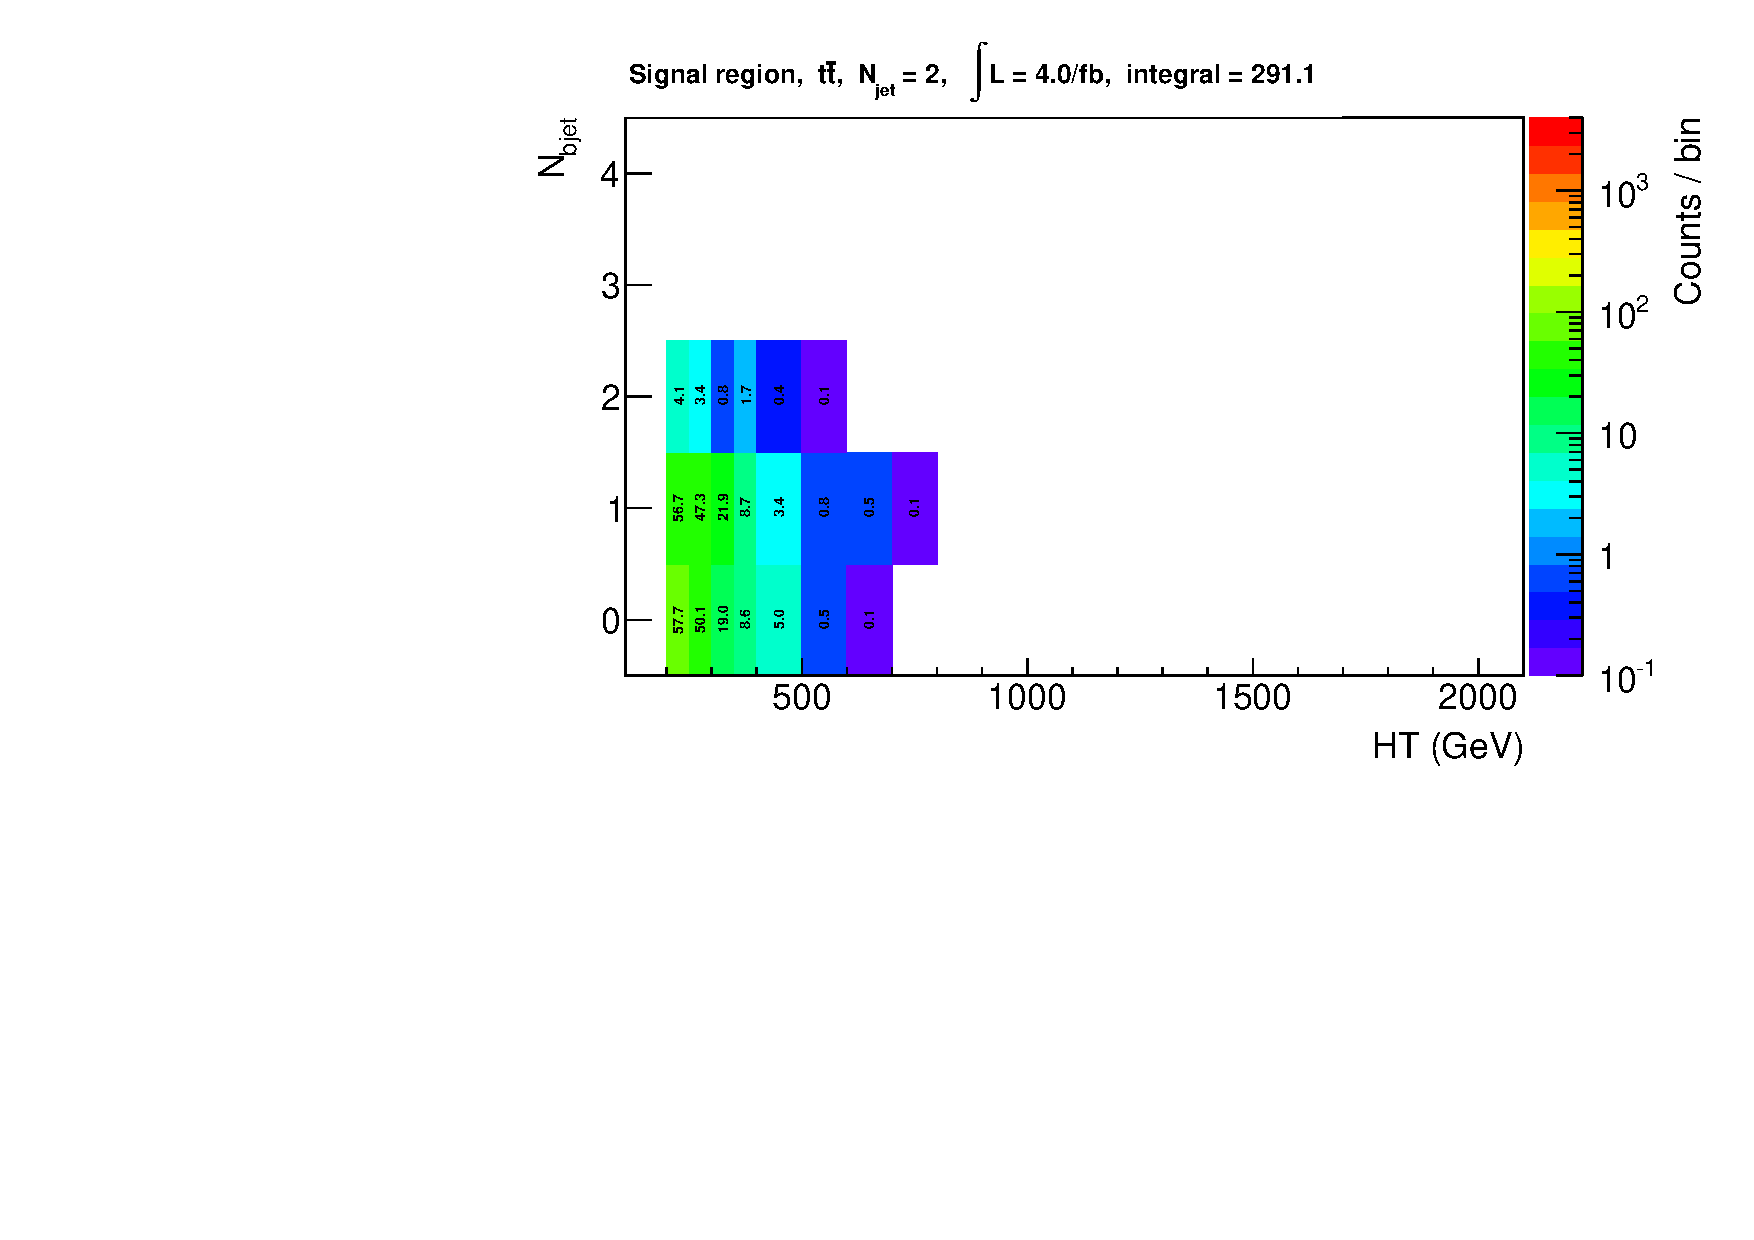
\includegraphics[width=0.5\textwidth]{figures/yieldPlots/had_ttbar_eq2j.pdf}
  }
  \caption{\label{fig:ewkYields1} Yields at $4\fbinv$ for the electroweak backgrounds in the
  hadronic signal region, $\njet=2$. The binning is chosen to be in line with the analysis
  bins. The contribution from the dominant backgrounds is shown separately.}
\end{figure}
\begin{figure}[]
  \centering
  \subfigure[Hadronic signal region yields for electroweak backgrounds
  ($\njet = 3$)]{
    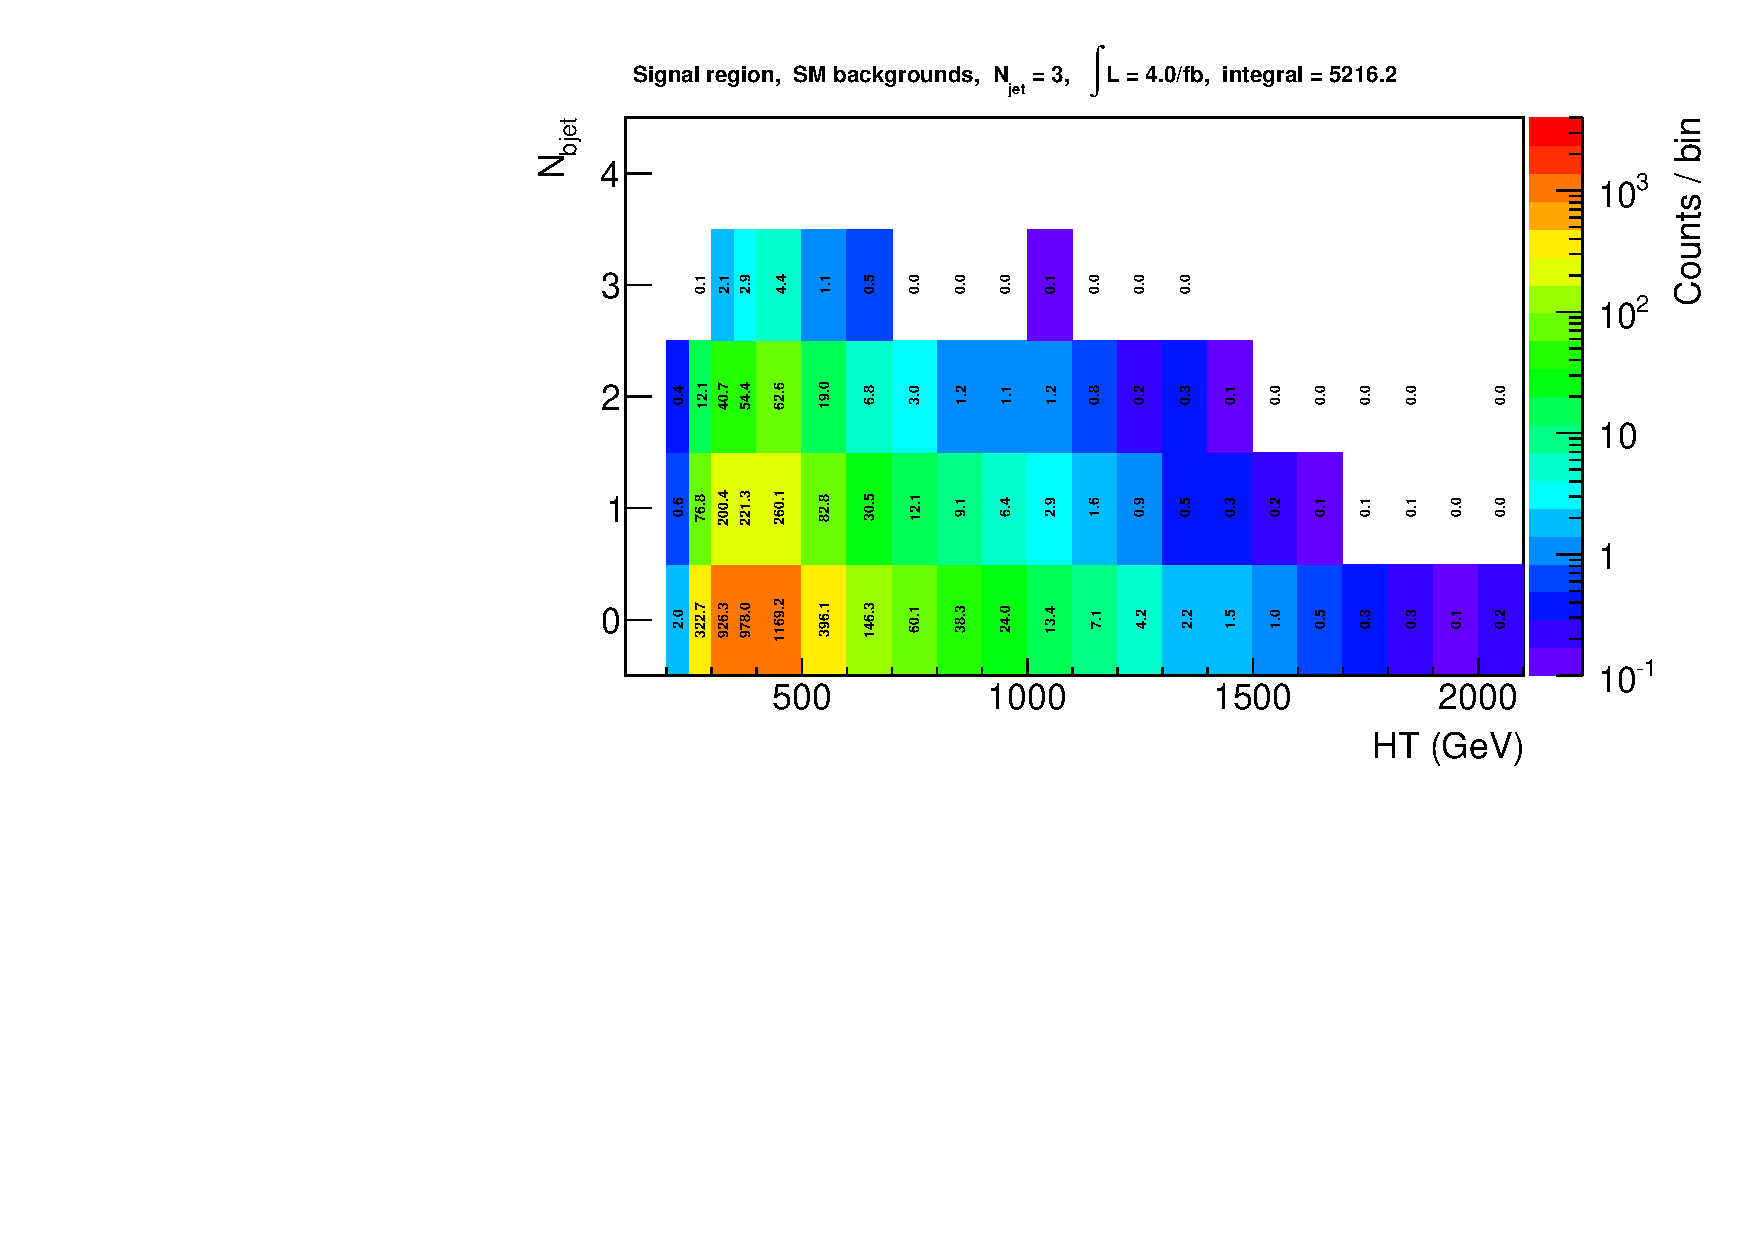
\includegraphics[width=0.5\textwidth]{figures/yieldPlots/had_ewk_eq3j.pdf}
  }~~
  \subfigure[Hadronic signal region yields for the \zInv background
  ($\njet = 3$)]{
    \includegraphics[width=0.5\textwidth]{figures/yieldPlots/had_zInv_eq3j.pdf}
  }\\
  \subfigure[Hadronic signal region yields for W~+~jets backtround
  ($\njet = 3$)]{
    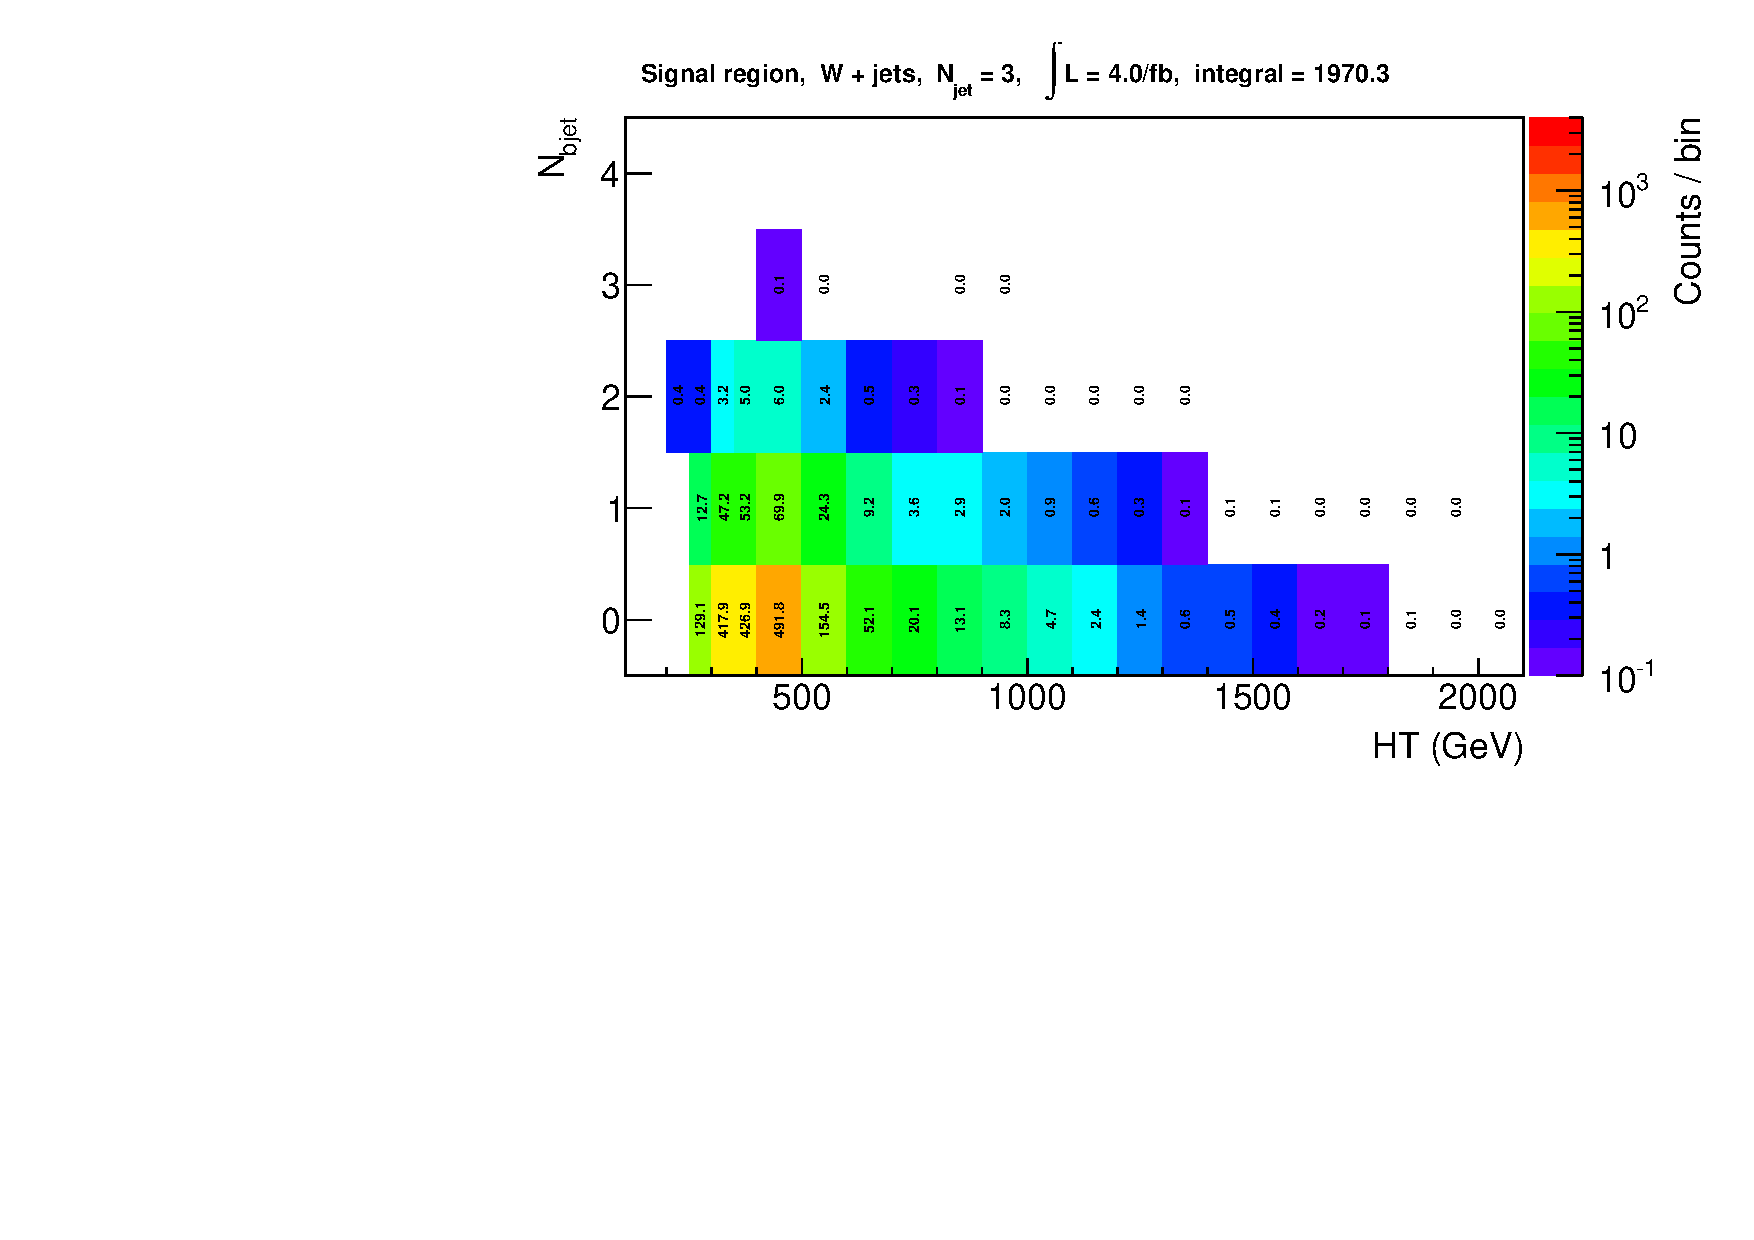
\includegraphics[width=0.5\textwidth]{figures/yieldPlots/had_wjets_eq3j.pdf}
  }~~
  \subfigure[Hadronic signal region yields for \ttbar background
  ($\njet = 3$)]{
    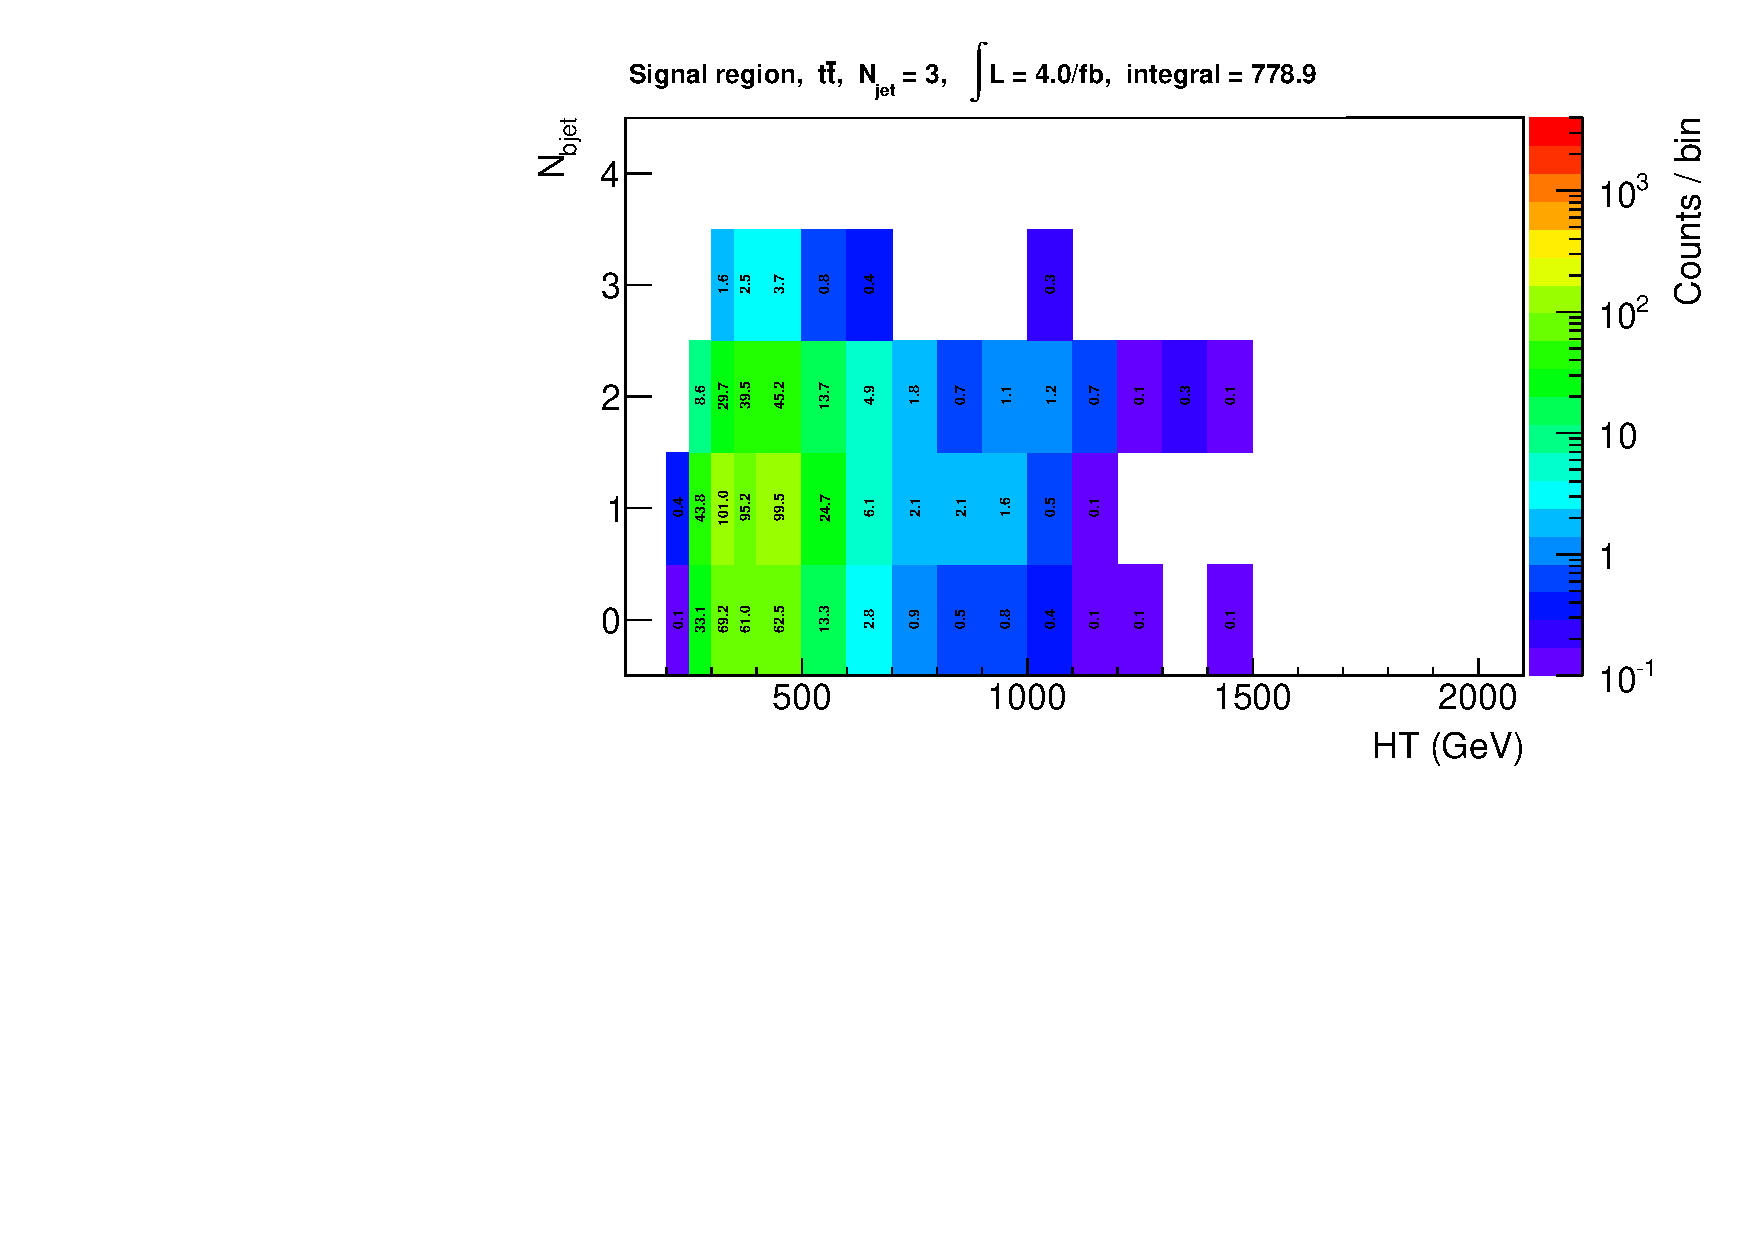
\includegraphics[width=0.5\textwidth]{figures/yieldPlots/had_ttbar_eq3j.pdf}
  }
  \caption{\label{fig:ewkYields2} Yields at $4\fbinv$ for the electroweak backgrounds in the
  hadronic signal region, $\njet=3$. The binning is chosen to be in line with the analysis
  bins. The contribution from the dominant backgrounds is shown separately.}
\end{figure}
\begin{figure}[]
  \centering
  \subfigure[Hadronic signal region yields for electroweak backgrounds
  ($\njet = 4$)]{
    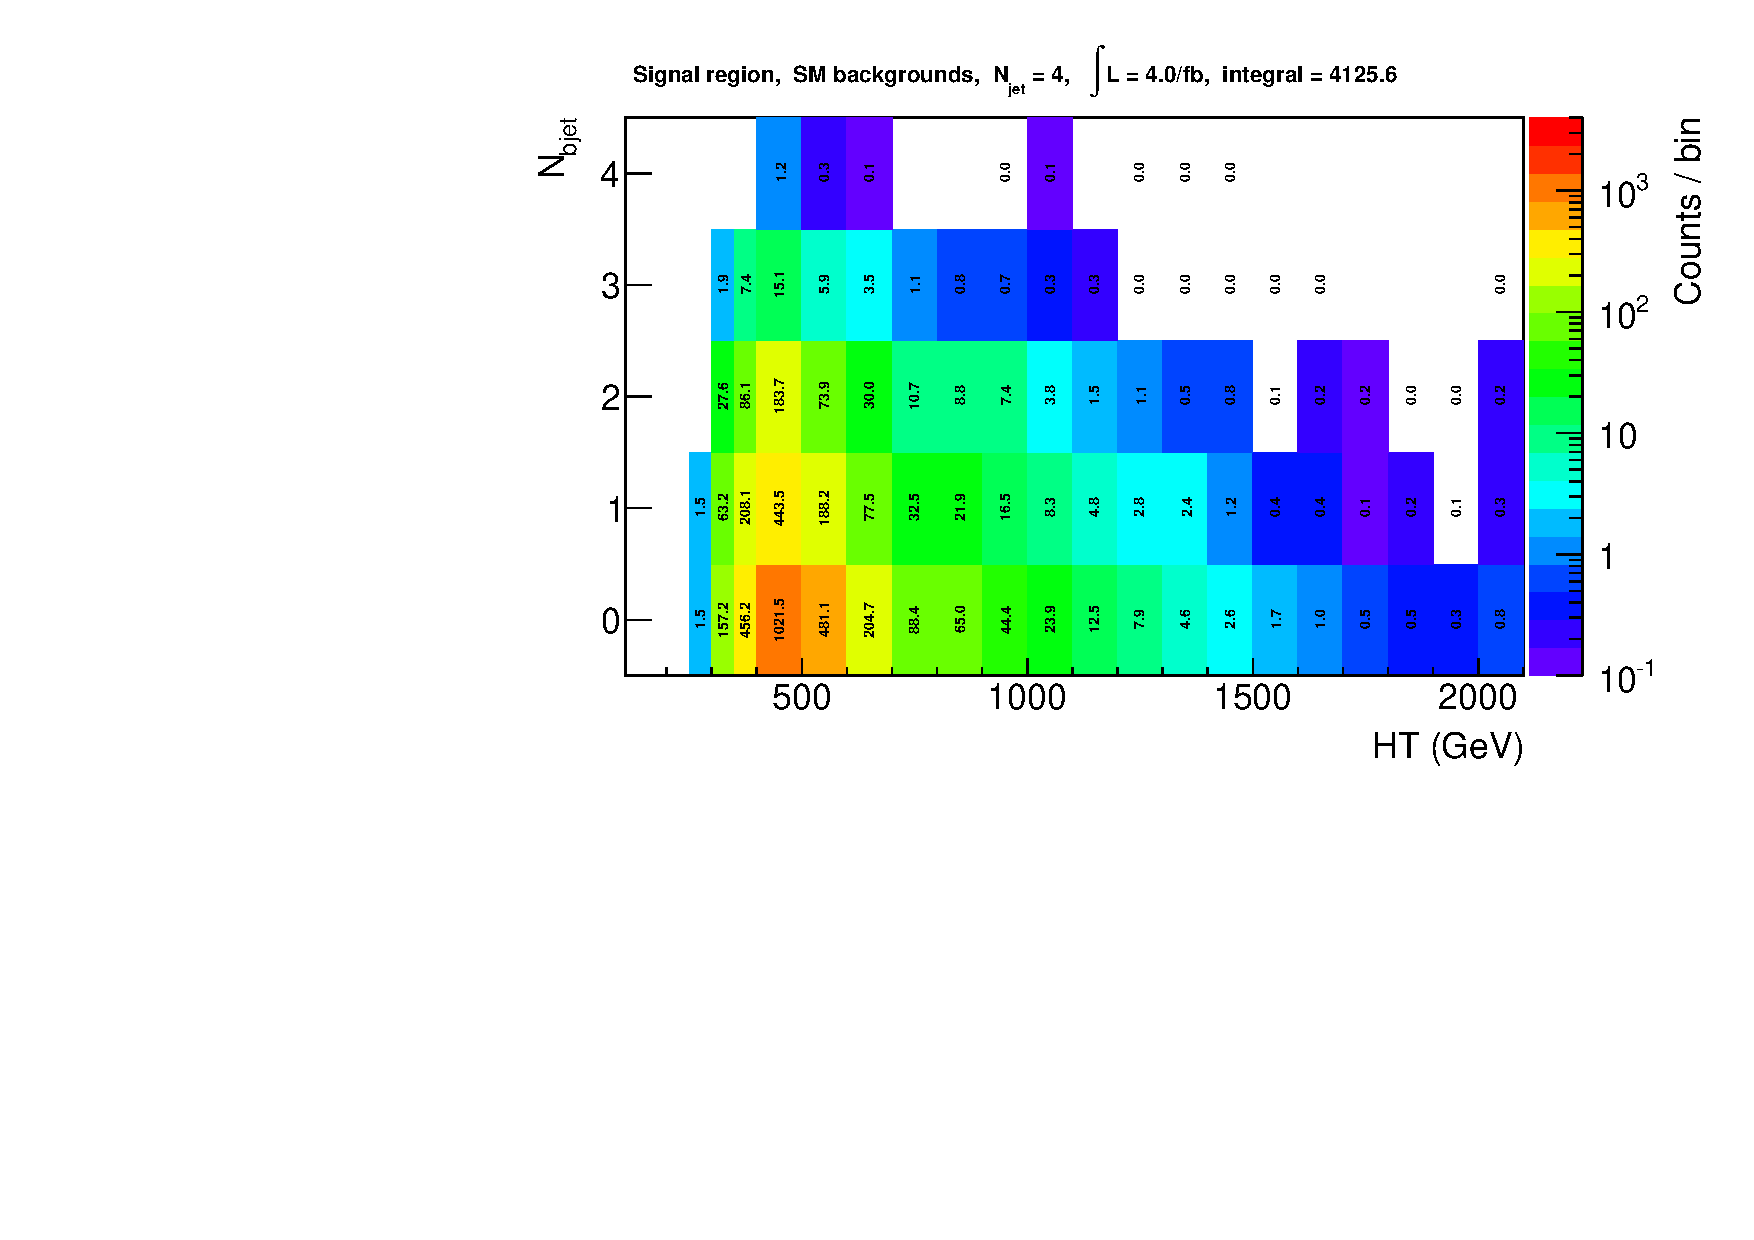
\includegraphics[width=0.5\textwidth]{figures/yieldPlots/had_ewk_eq4j.pdf}
  }~~
  \subfigure[Hadronic signal region yields for the \zInv background
  ($\njet = 4$)]{
    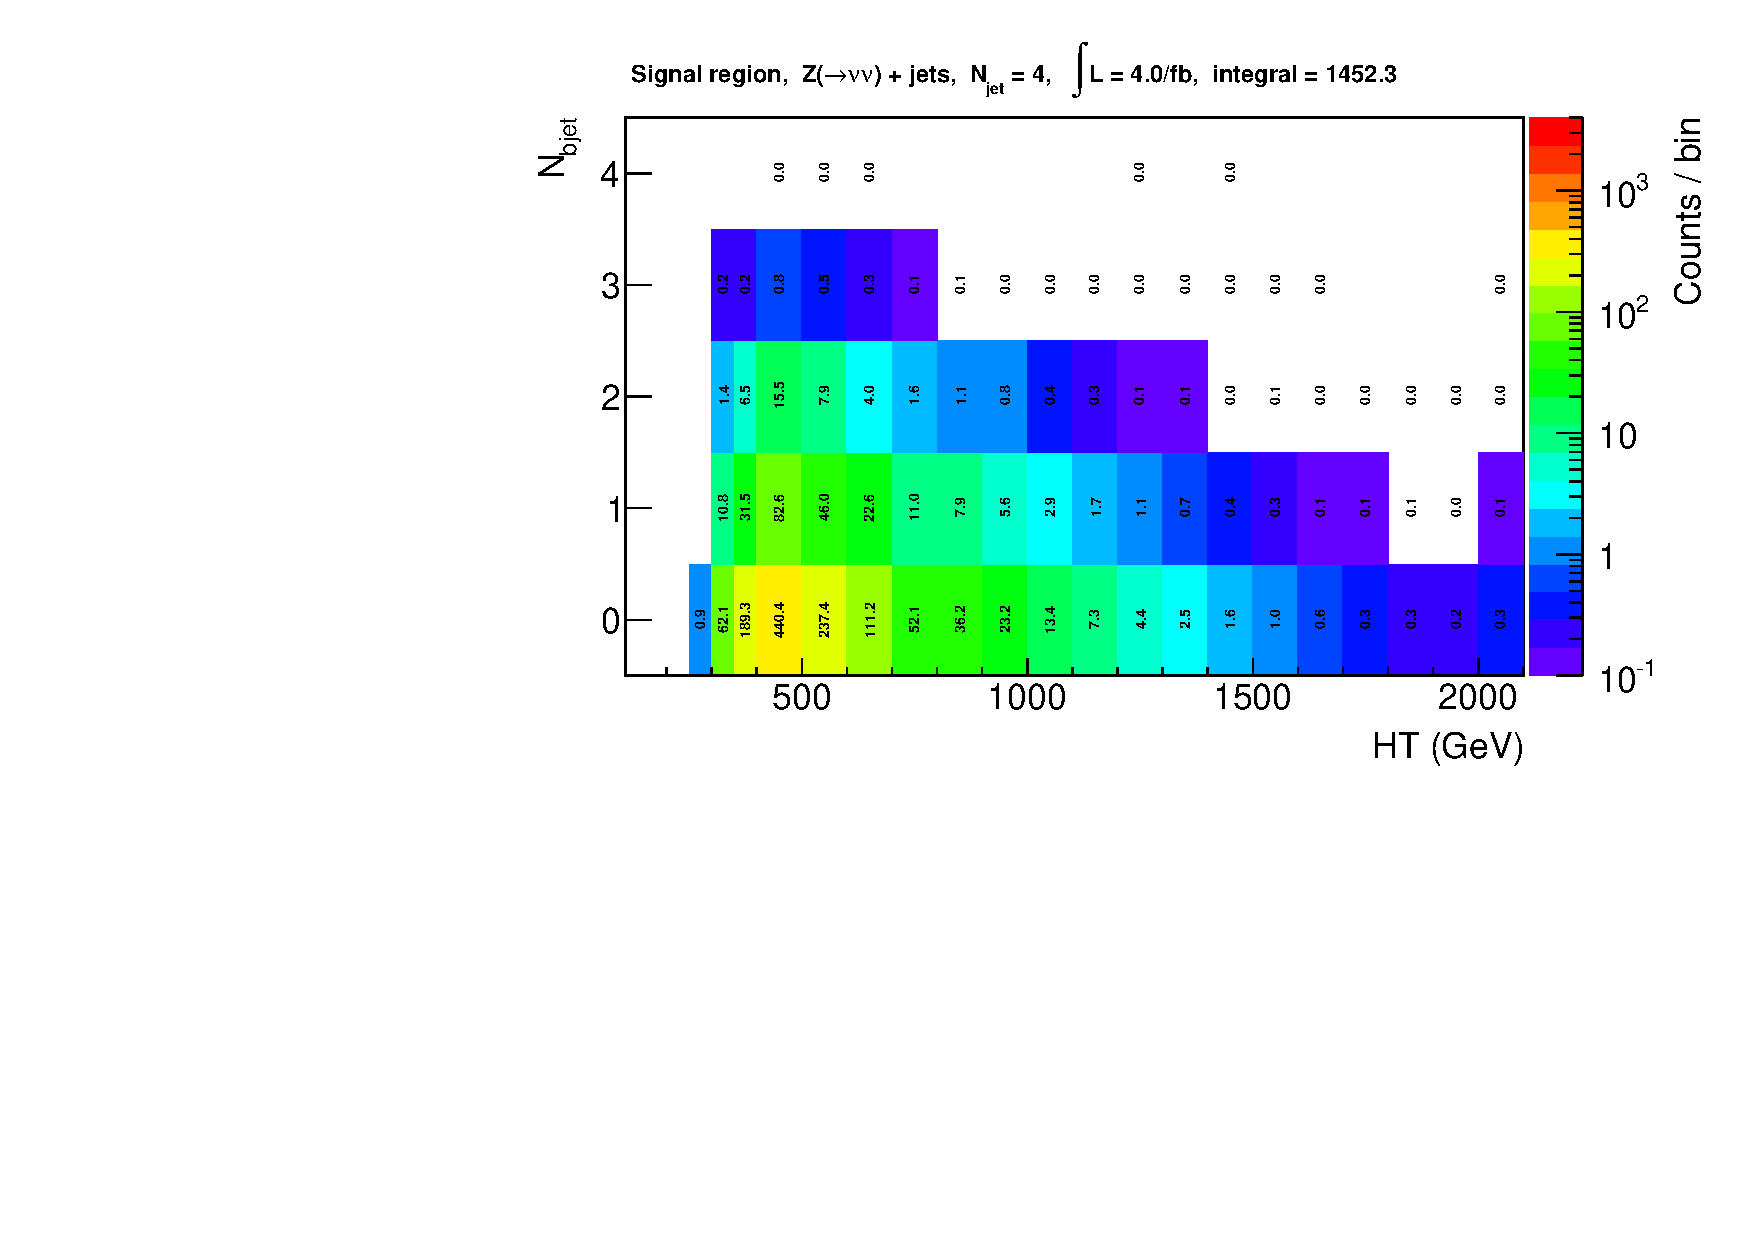
\includegraphics[width=0.5\textwidth]{figures/yieldPlots/had_zinv_eq4j.pdf}
  }\\
  \subfigure[Hadronic signal region yields for W~+~jets backtround
  ($\njet = 4$)]{
    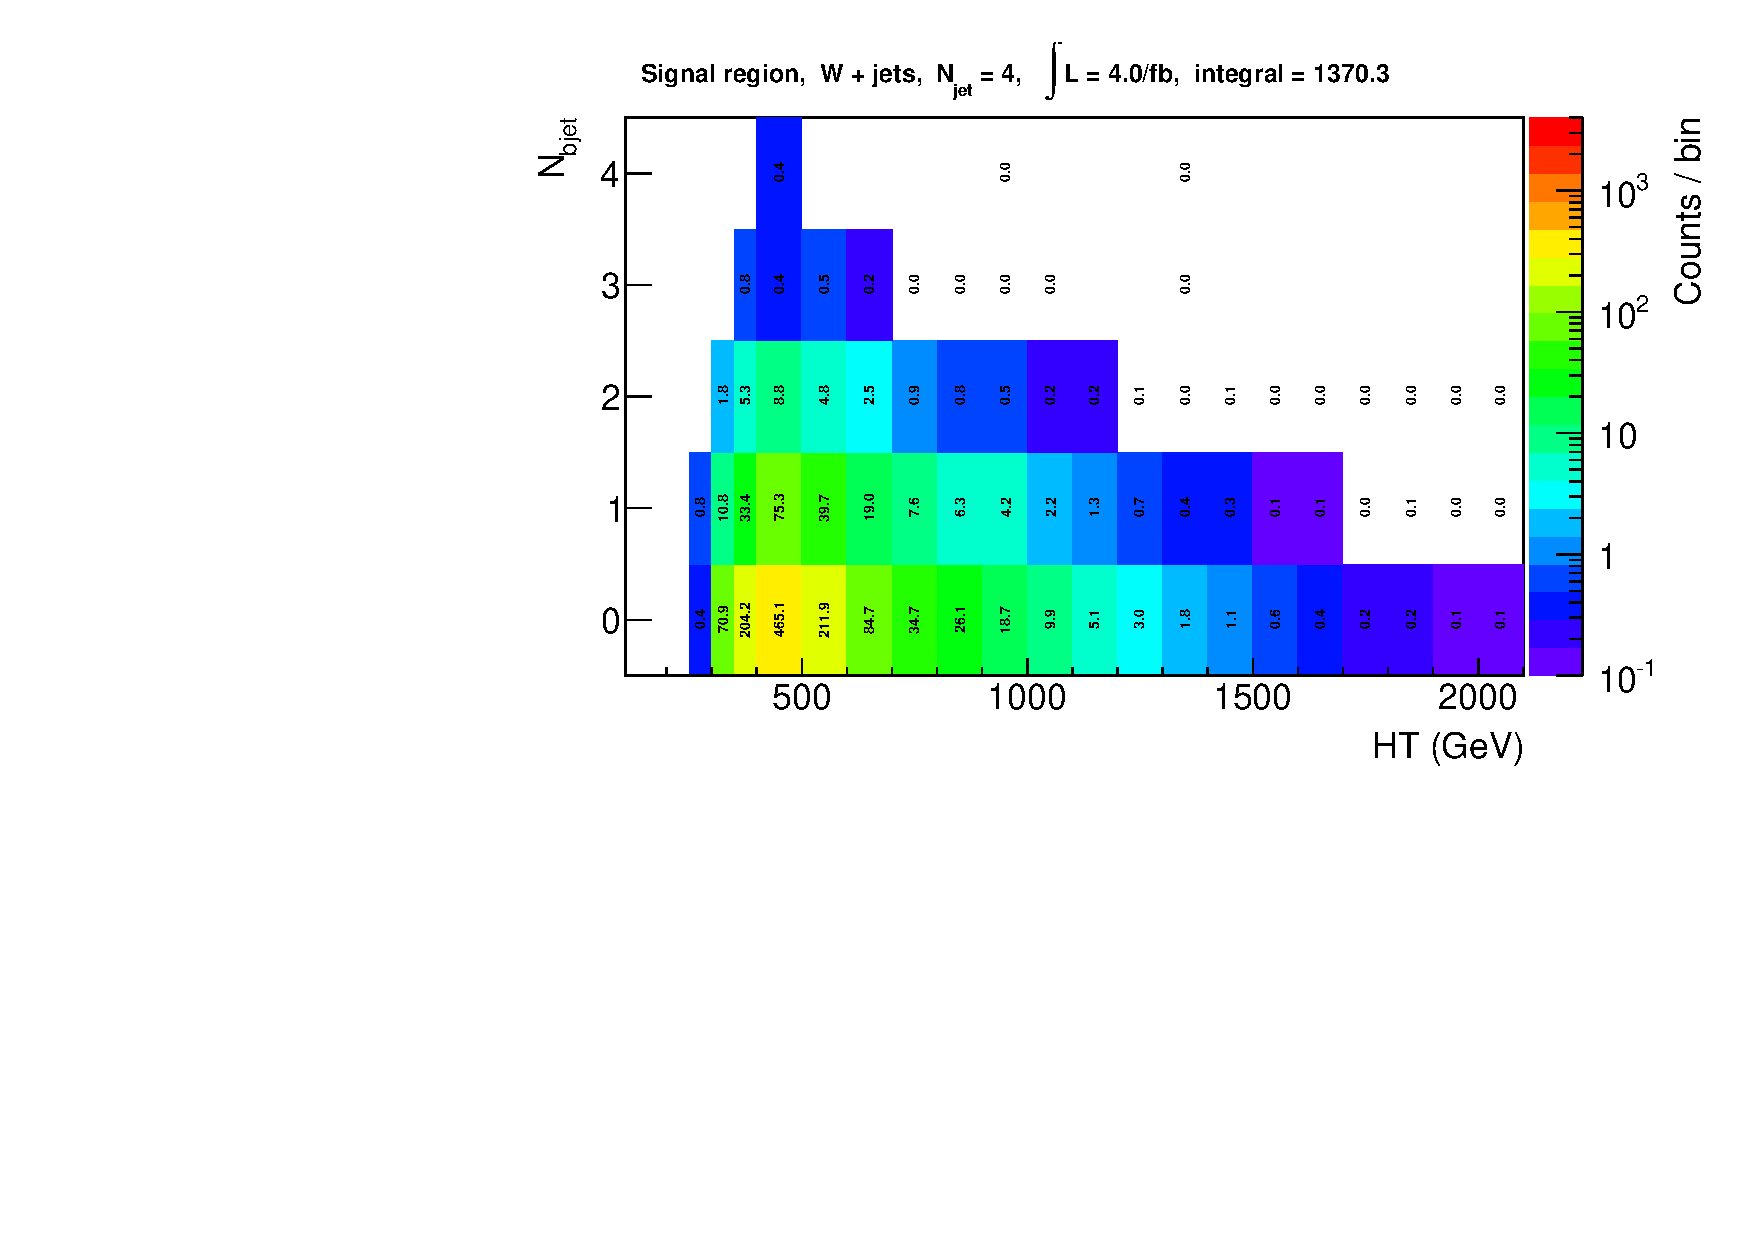
\includegraphics[width=0.5\textwidth]{figures/yieldPlots/had_wjets_eq4j.pdf}
  }~~
  \subfigure[Hadronic signal region yields for \ttbar background
  ($\njet = 4$)]{
    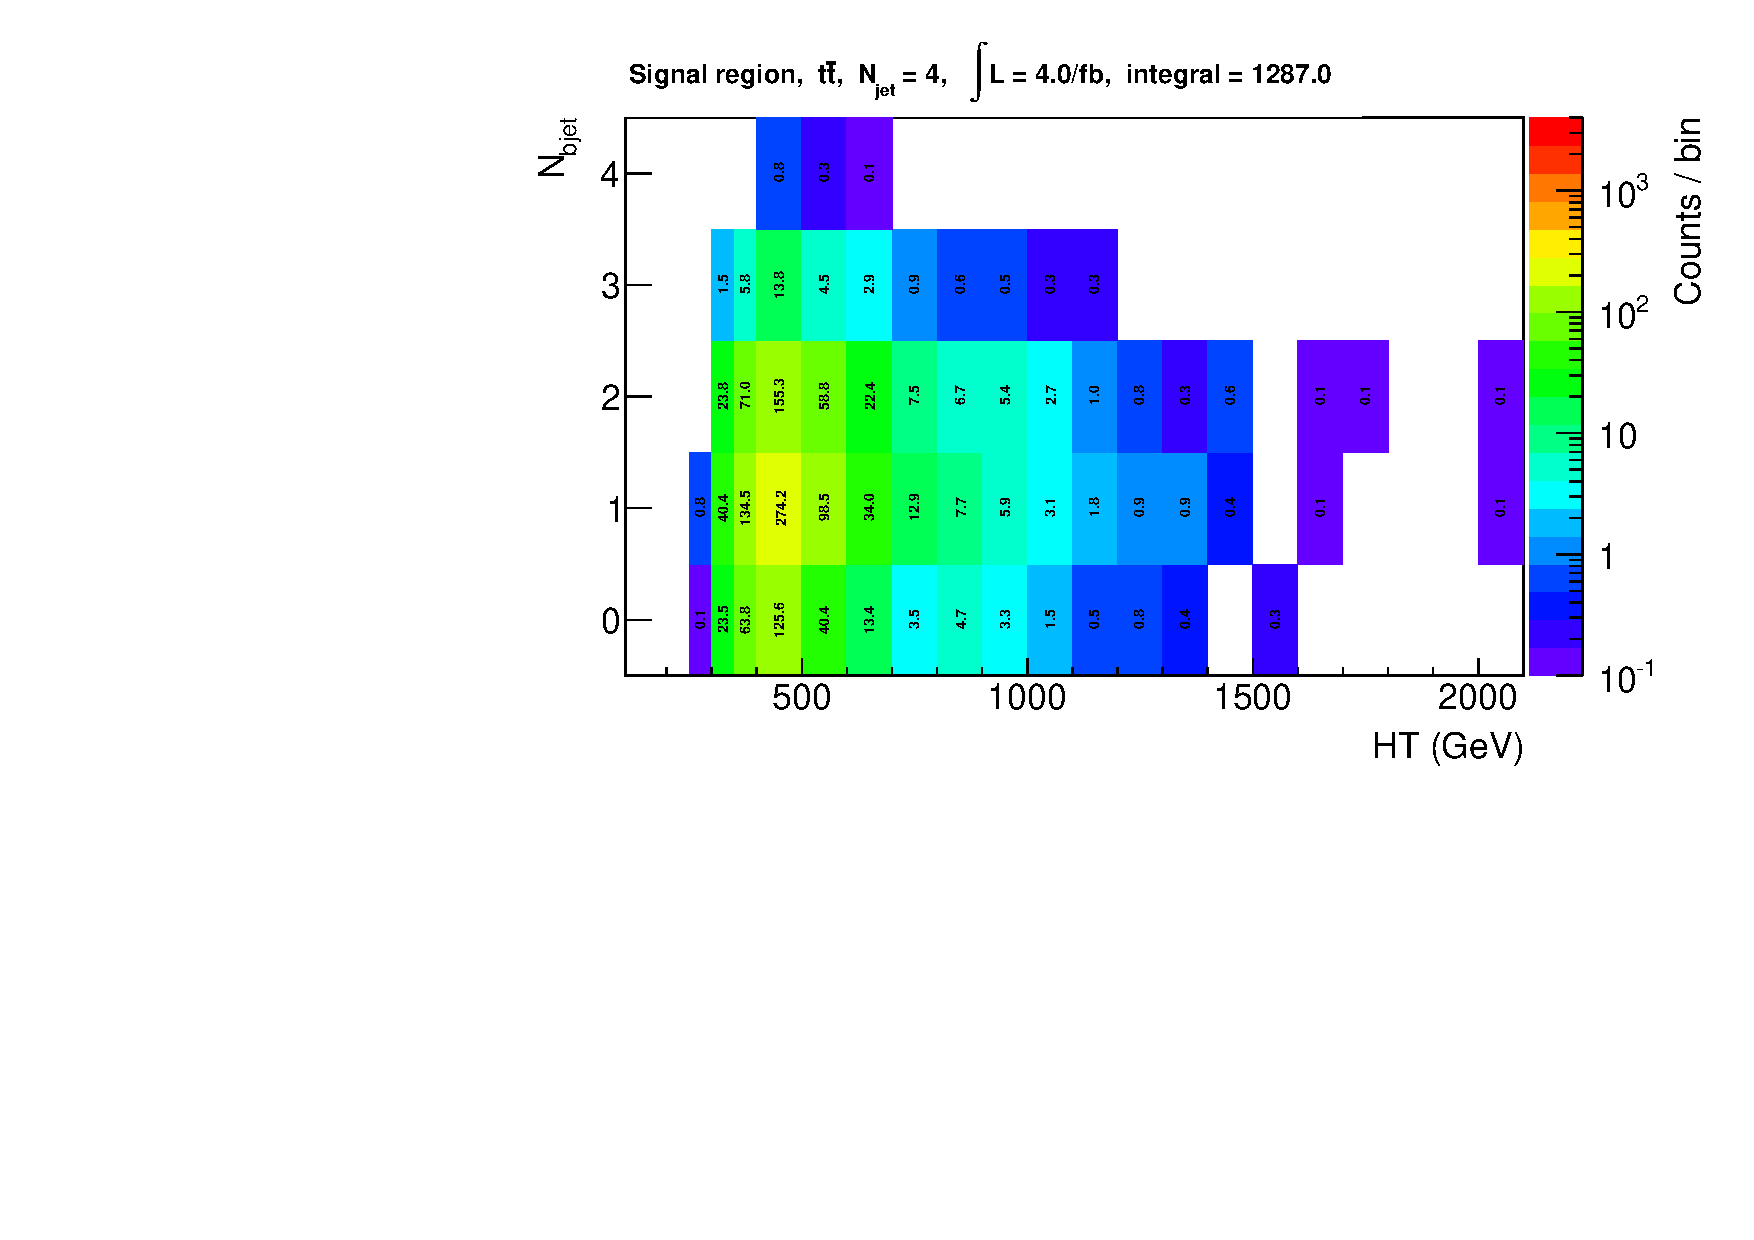
\includegraphics[width=0.5\textwidth]{figures/yieldPlots/had_ttbar_eq4j.pdf}
  }
  \caption{\label{fig:ewkYields3} Yields at $4\fbinv$ for the electroweak backgrounds in the
  hadronic signal region, $\njet=4$. The binning is chosen to be in line with the analysis
  bins. The contribution from the dominant backgrounds is shown separately.}
\end{figure}
\begin{figure}[]
  \centering
  \subfigure[Hadronic signal region yields for electroweak backgrounds
  ($\njet \geq 5$)]{
    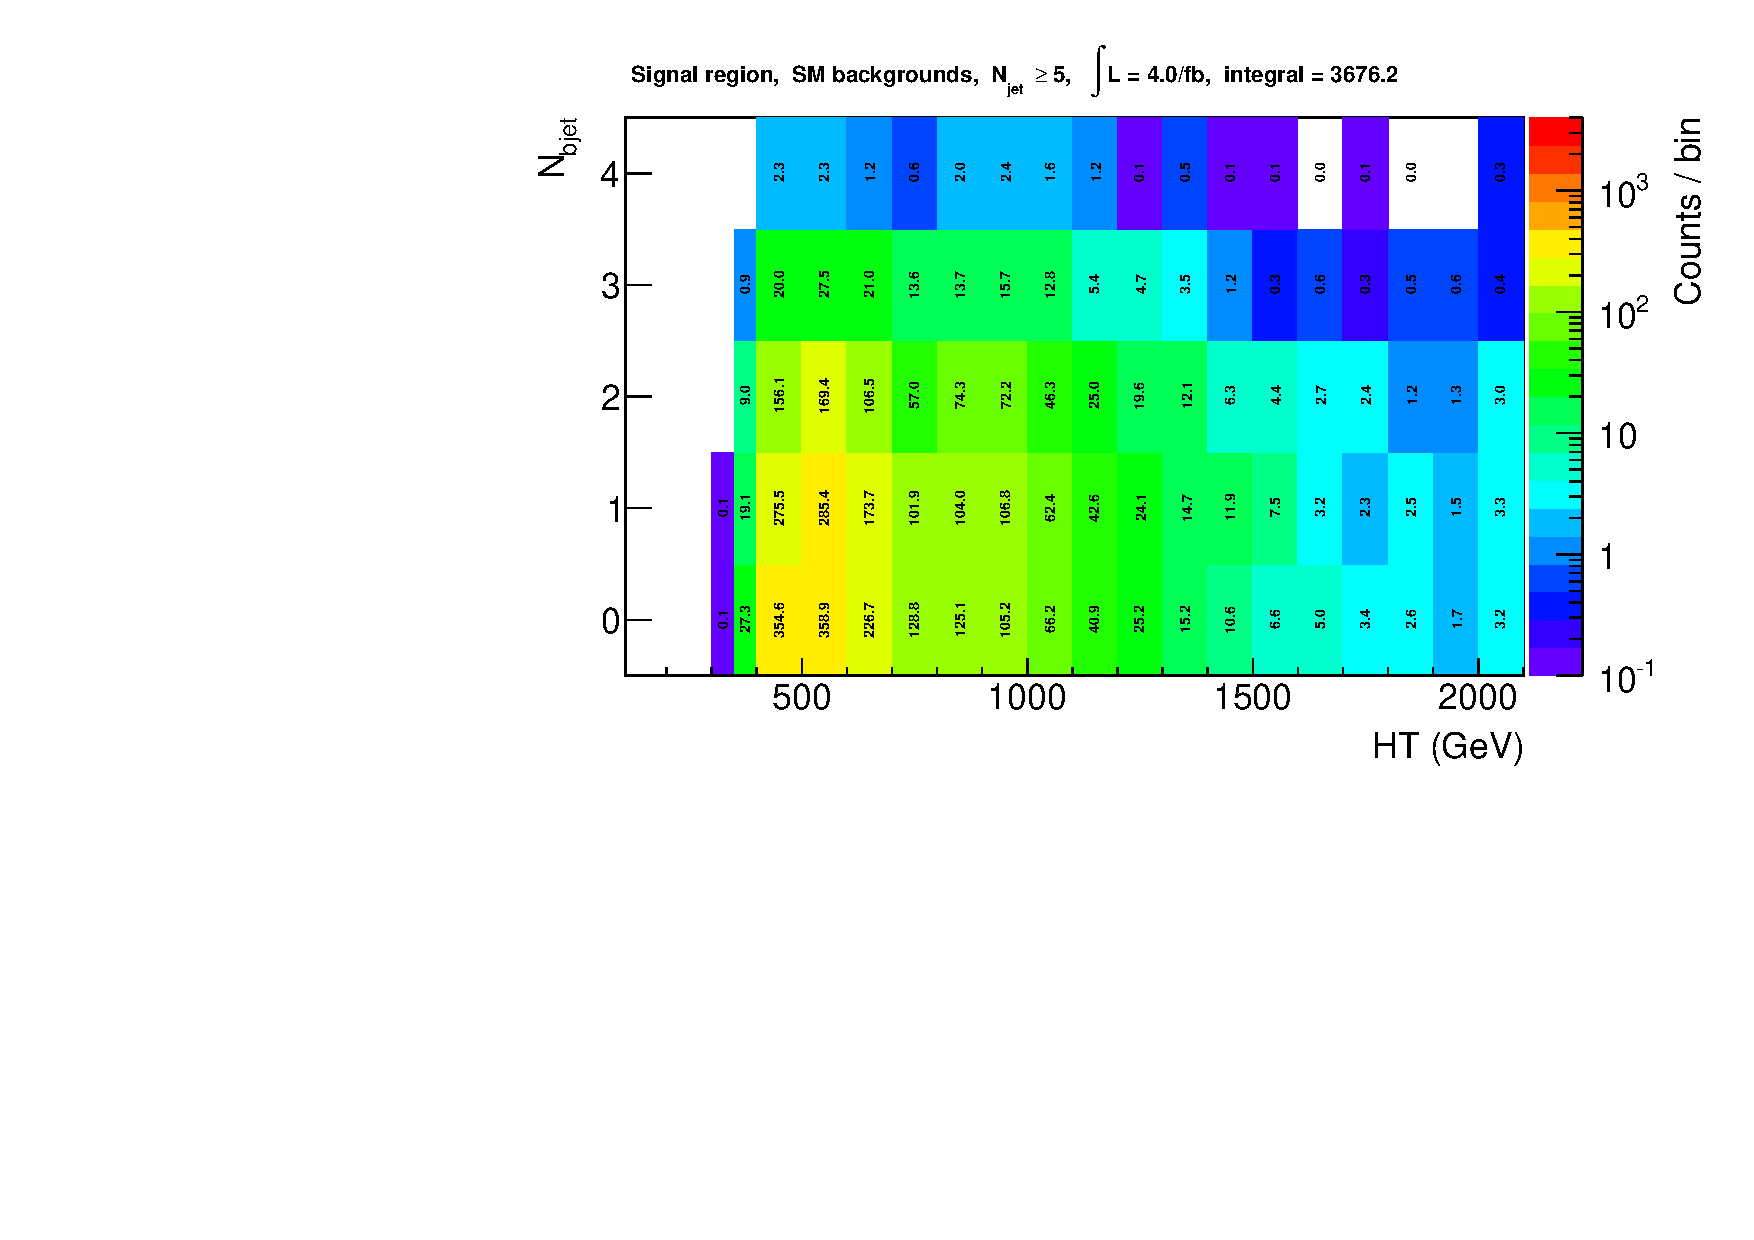
\includegraphics[width=0.5\textwidth]{figures/yieldPlots/had_ewk_ge5j.pdf}
  } ~~
  \subfigure[Hadronic signal region yields for the \zInv background
  ($\njet \geq 5$)]{
    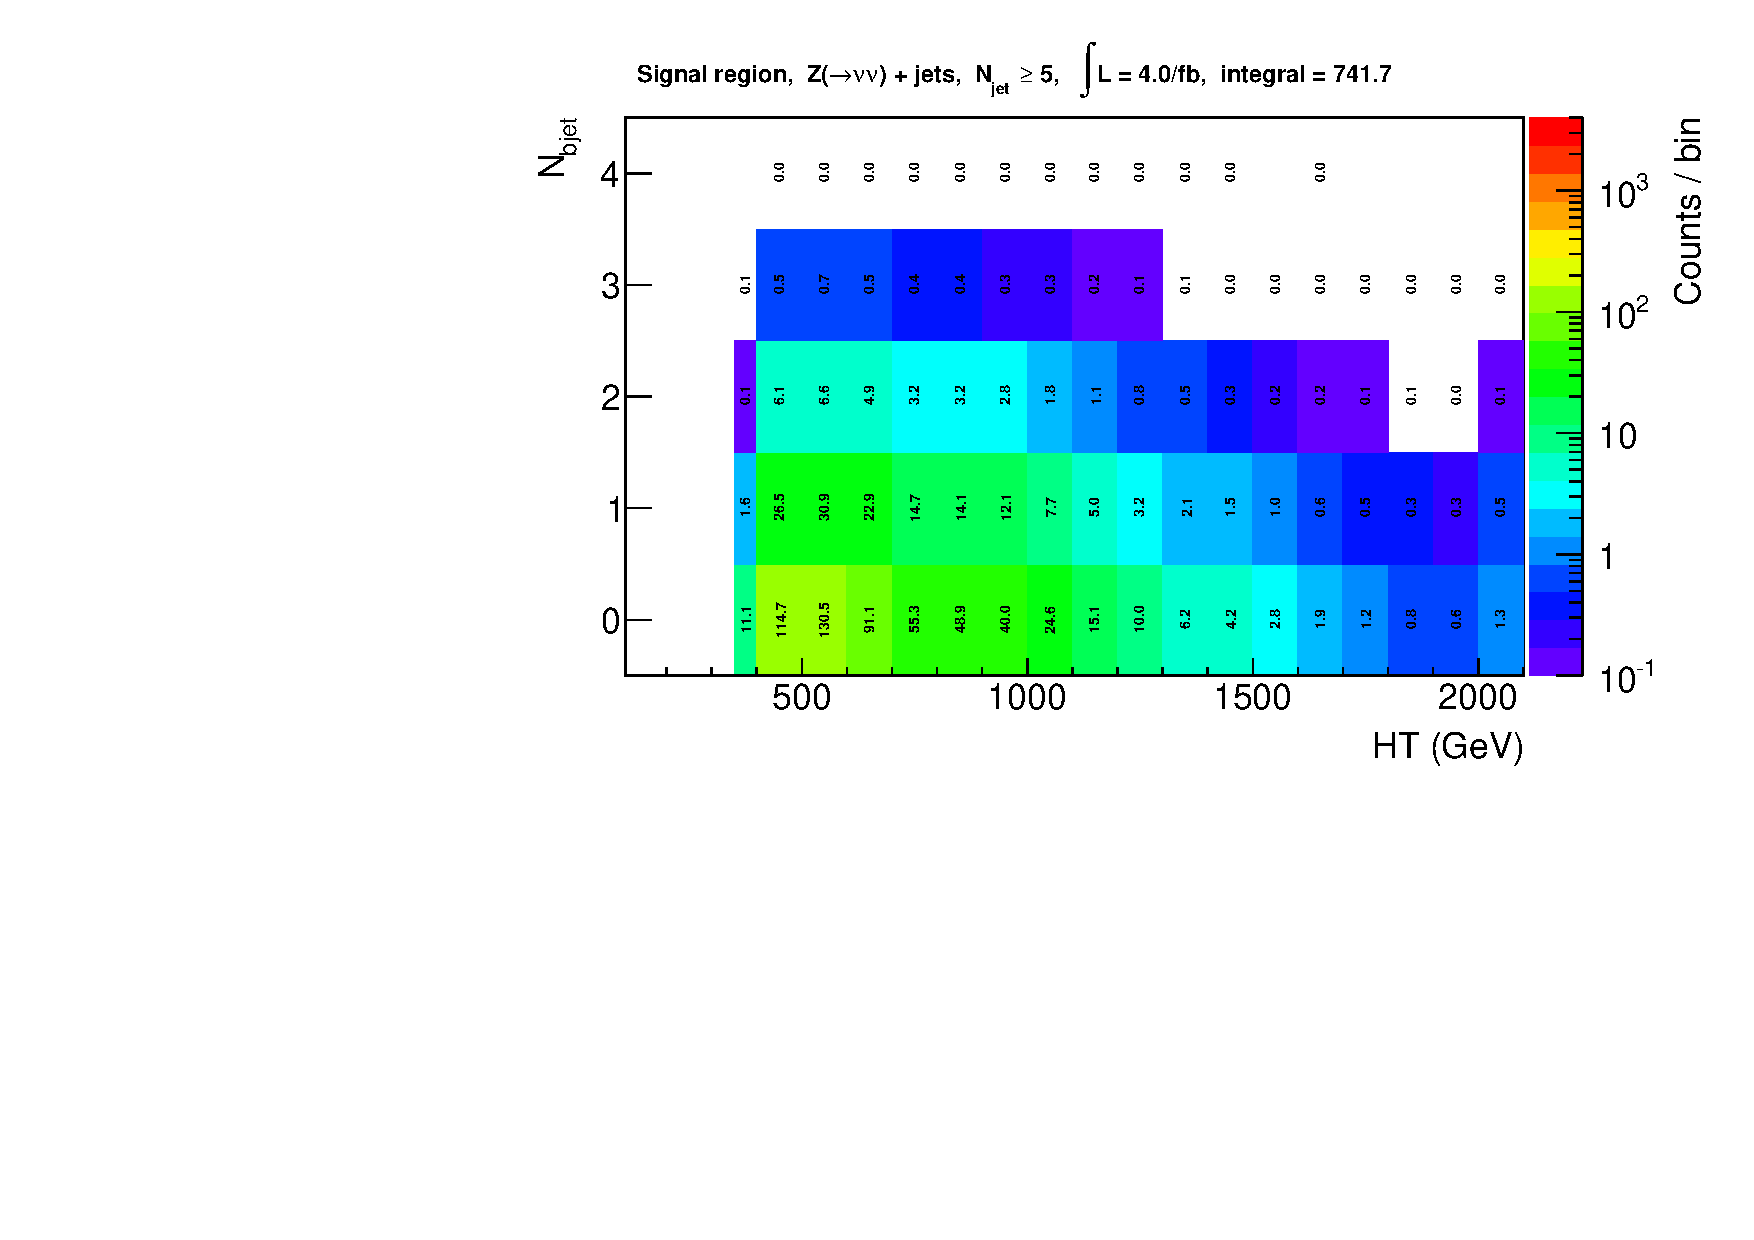
\includegraphics[width=0.5\textwidth]{figures/yieldPlots/had_zinv_ge5j.pdf}
  }\\
  \subfigure[Hadronic signal region yields for W~+~jets backtround
  ($\njet \geq 5$)]{
    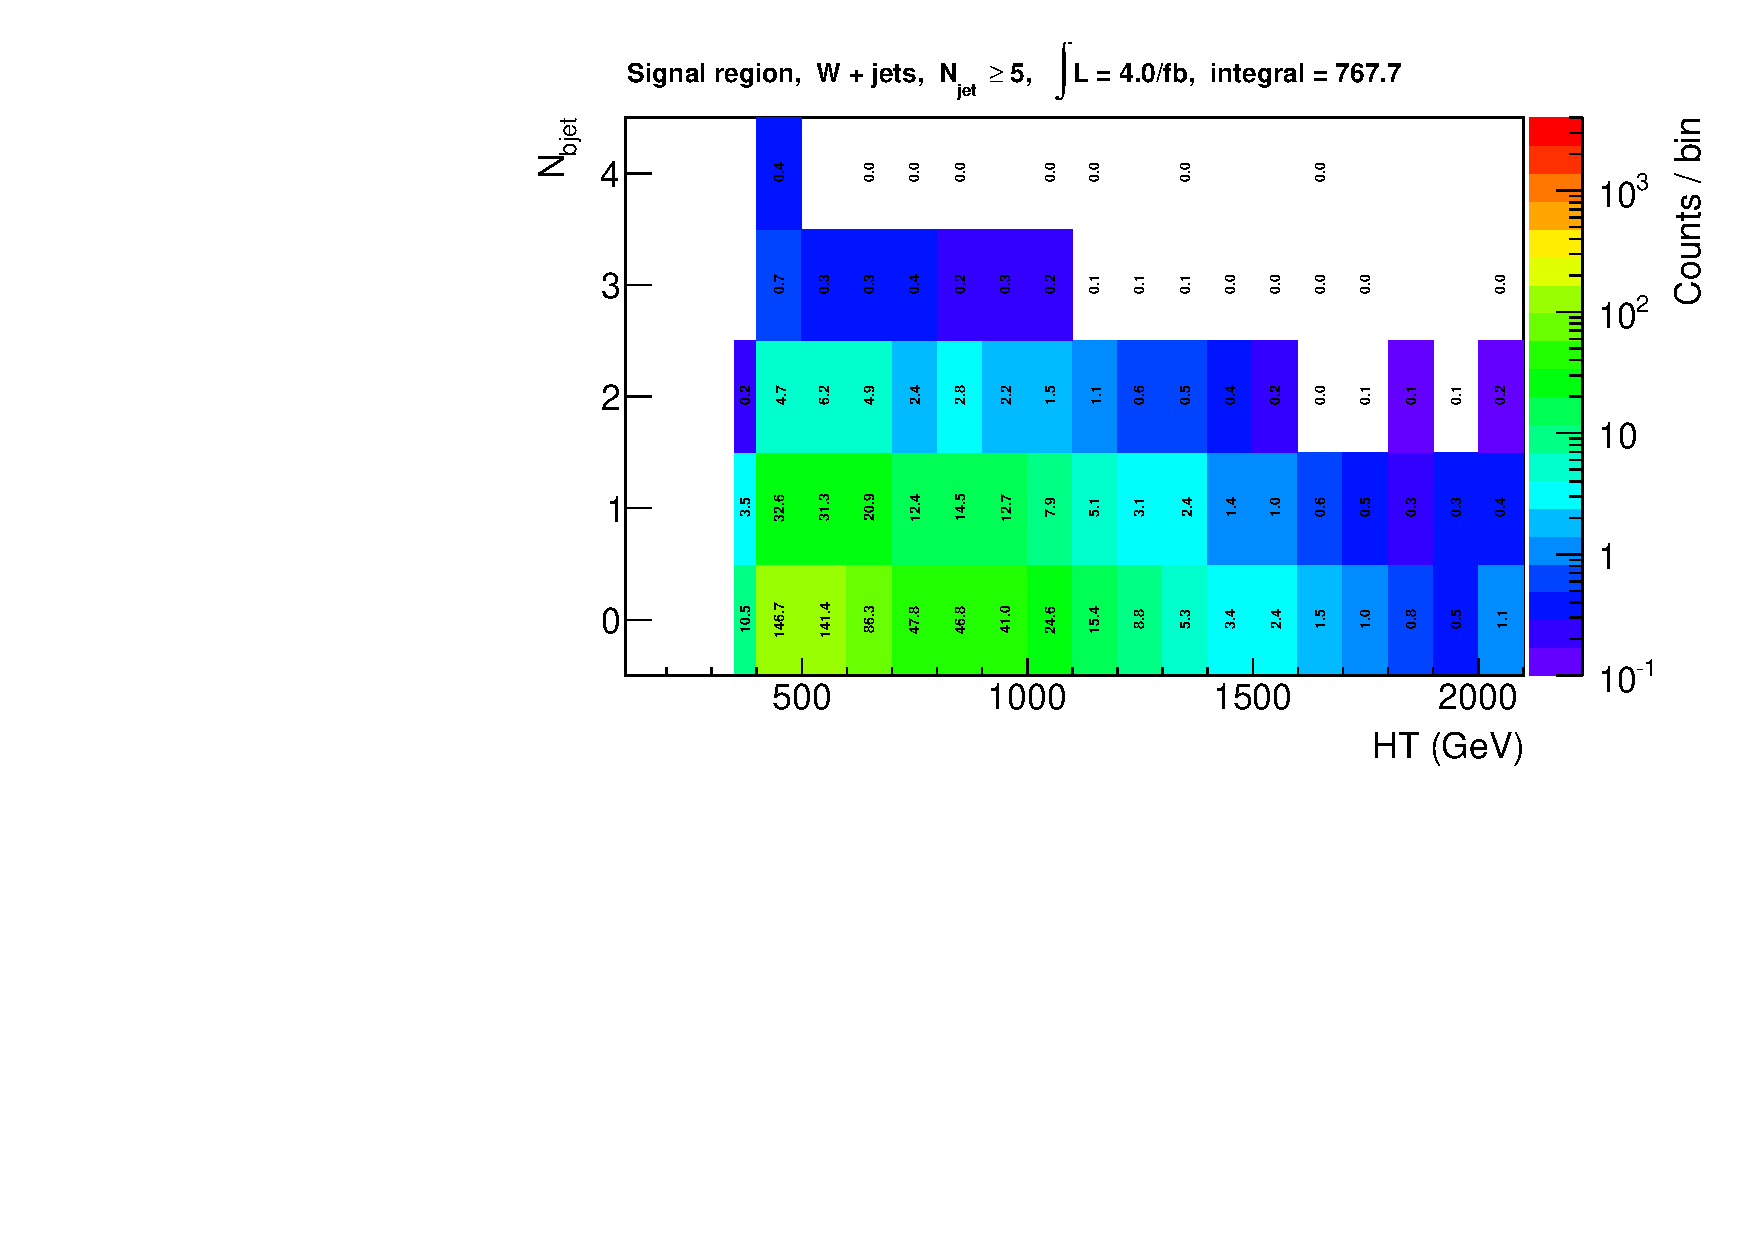
\includegraphics[width=0.5\textwidth]{figures/yieldPlots/had_wjets_ge5j.pdf}
  }~~
  \subfigure[Hadronic signal region yields for \ttbar background
  ($\njet \geq 5$)]{
    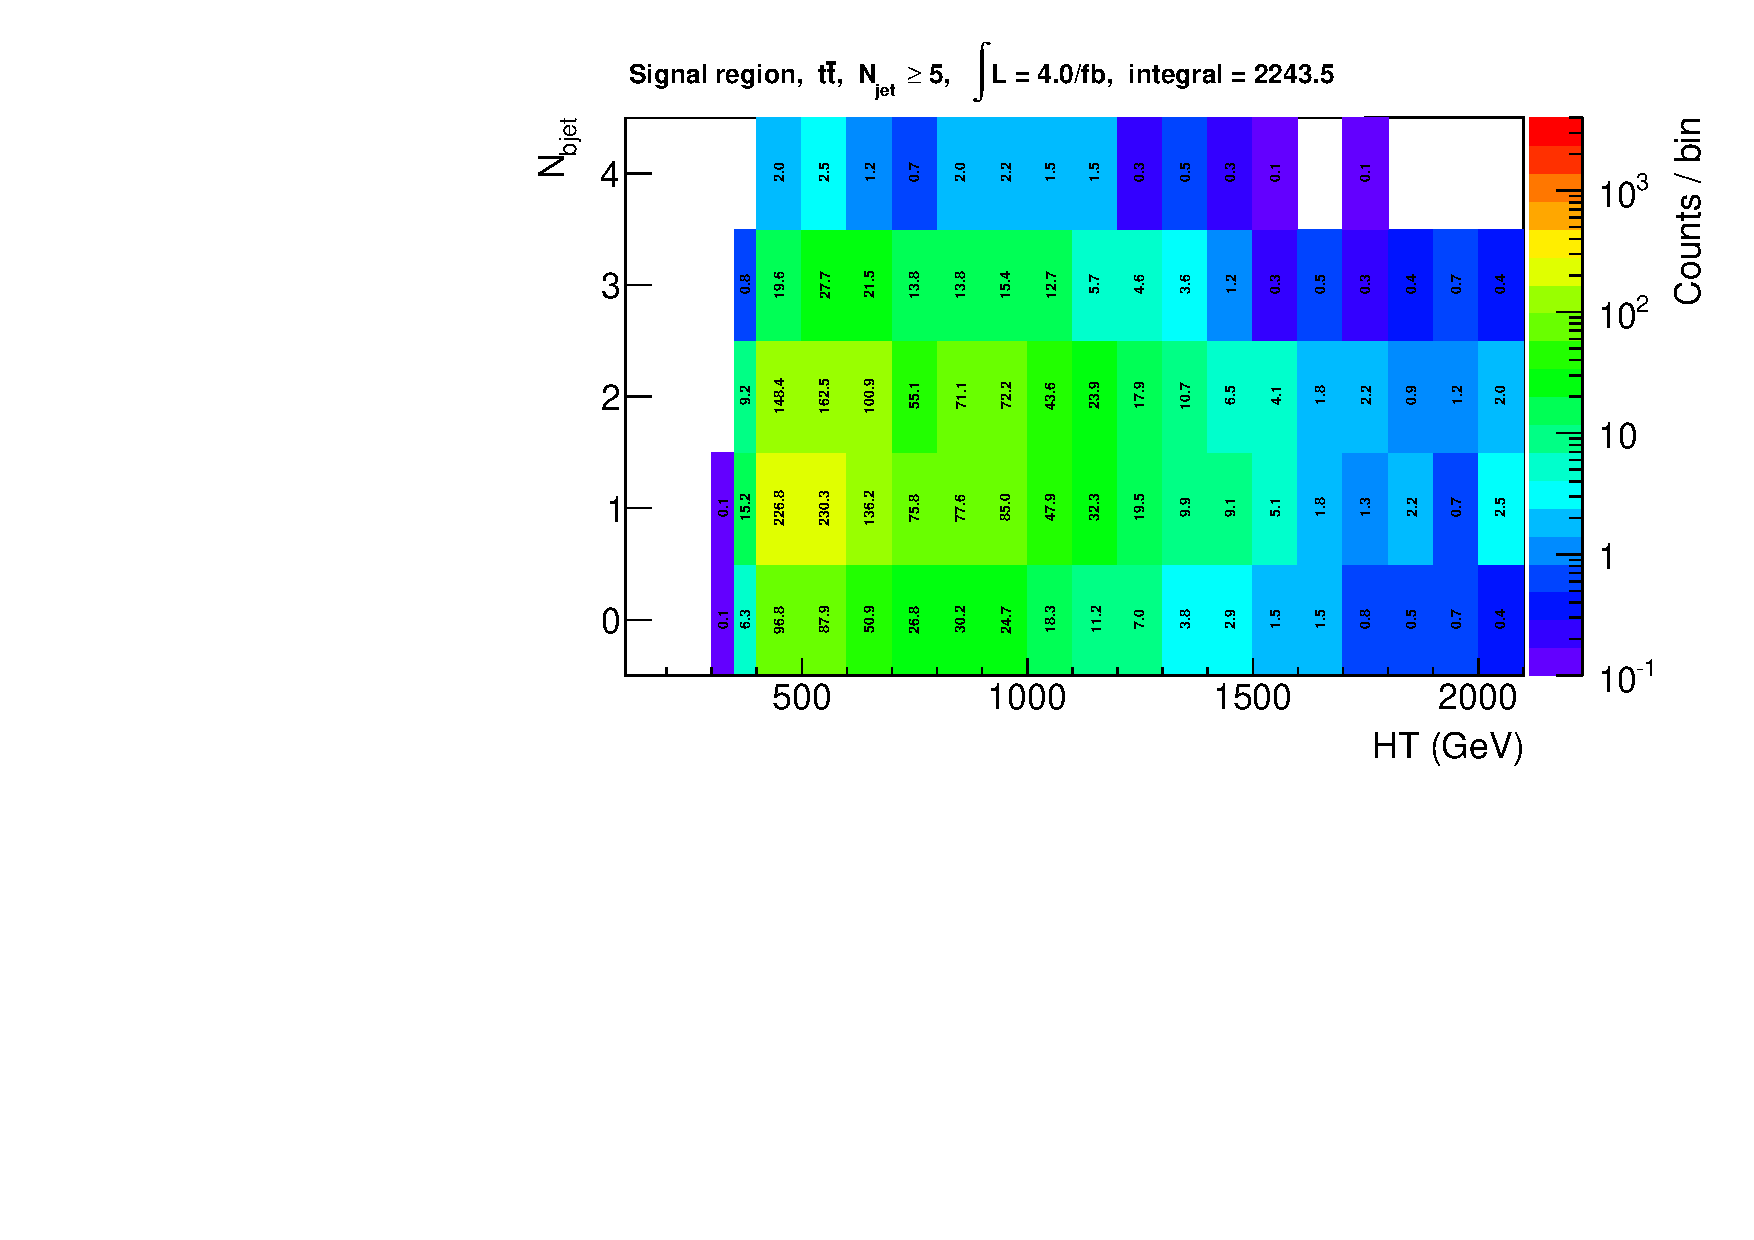
\includegraphics[width=0.5\textwidth]{figures/yieldPlots/had_ttbar_ge5j.pdf}
  }

  \\
  \subfigure[Hadronic signal region yields for T1bbbb simplified model
  \label{fig:sigYields}
  ($\njet \geq 5$)]{
    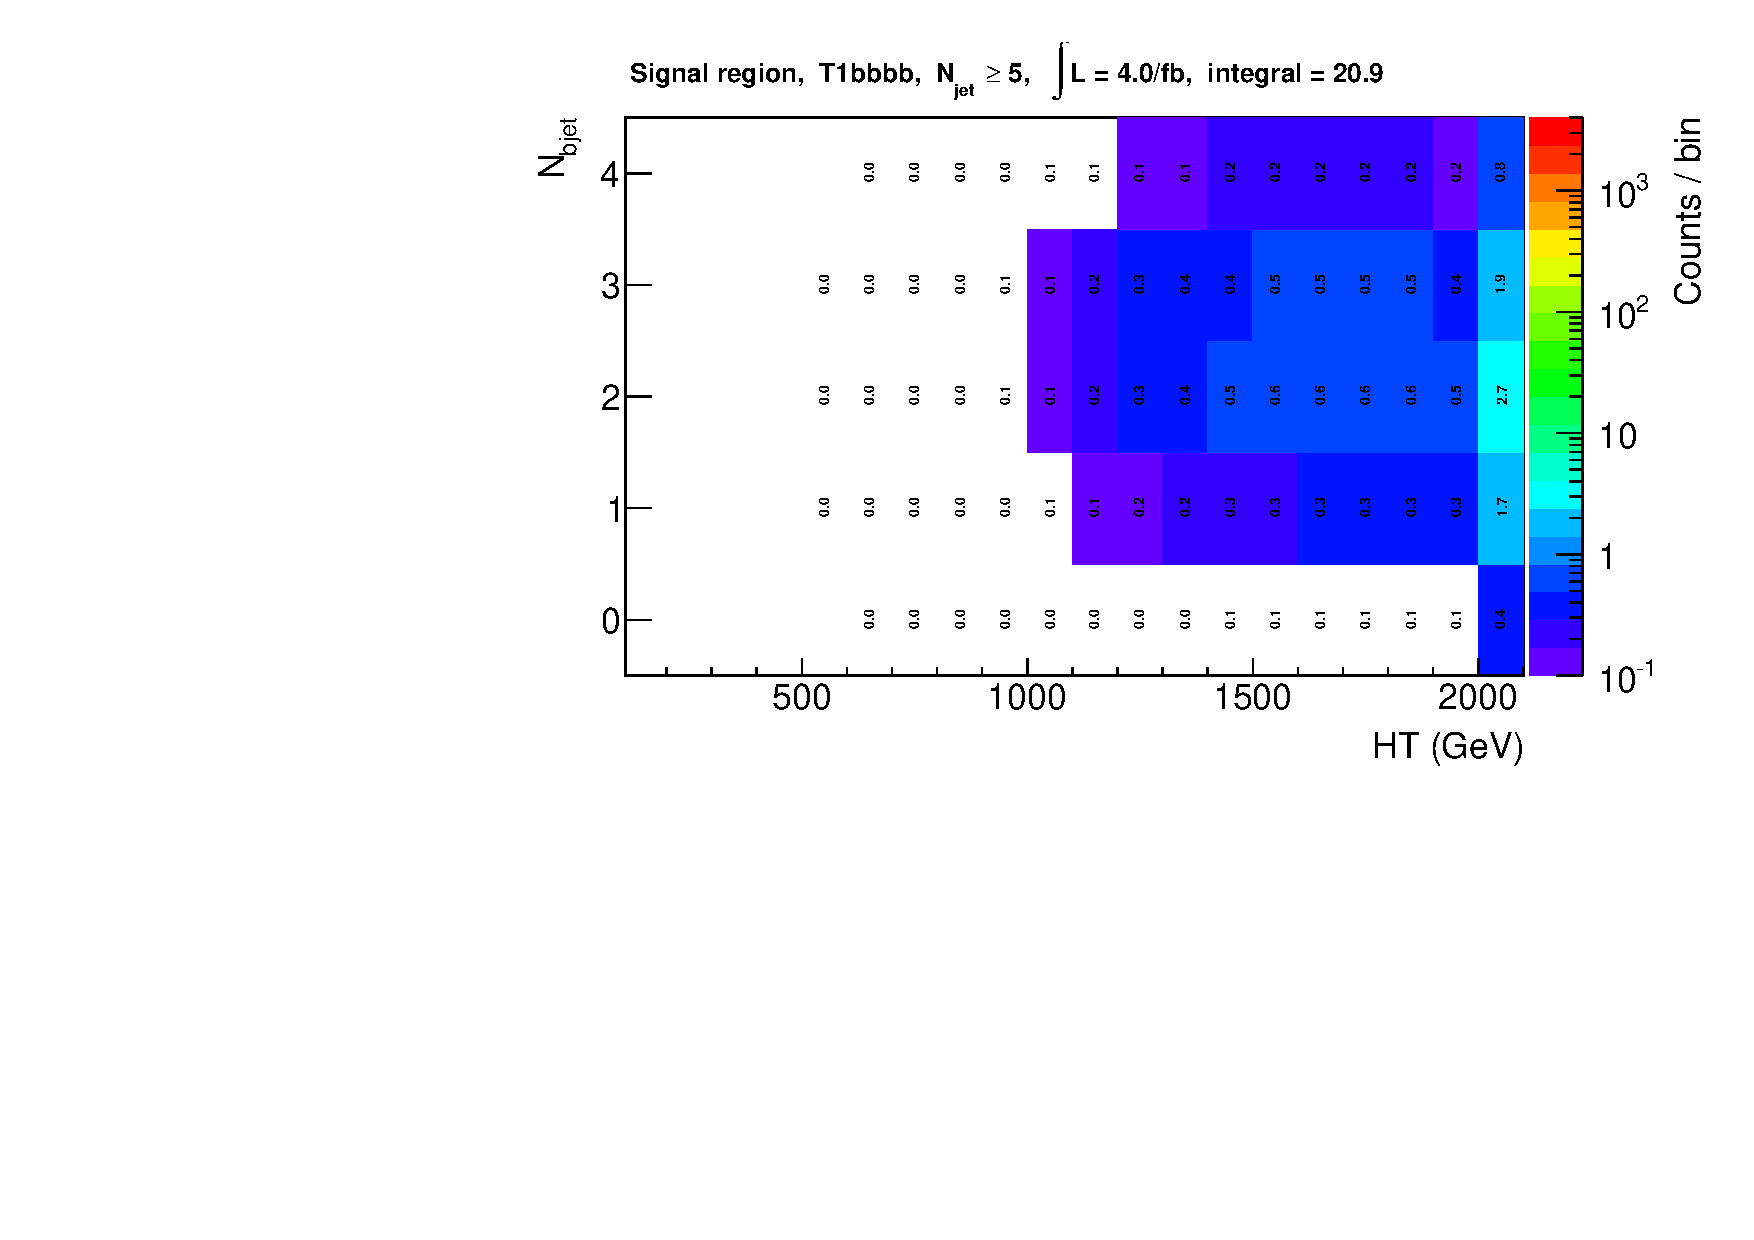
\includegraphics[width=0.5\textwidth]{figures/yieldPlots/sig_T1bbbb_ge5j.pdf}
  }
  \\
  \caption{\label{fig:ewkYields4} Yields at $4\fbinv$ for the electroweak backgrounds in the
  hadronic signal region, $\njet\geq5$. The binning is chosen to be in line with the analysis
  bins. The contribution from the dominant backgrounds is shown separately.}
\end{figure}

%%____________________________________________________________________________||
\subsection{Yields in the control samples}

The yields in the \mj, \mmj and \gj control samples can be seen in
Figures~\ref{fig:muYields}, \ref{fig:mumuYields} and \ref{fig:gammaYields}
respectively. The number of events in each of these bins is important for
working out how far we can extend in our analysis bins. We require there to be
enough events in the control samples to allow robust data driven prediction of
the backgrounds.

\begin{figure}[h!]
  \centering
  \subfigure[Yields from \texorpdfstring{\mj}{muon plus jets} control sample
  ($\njet = 2$)]{
    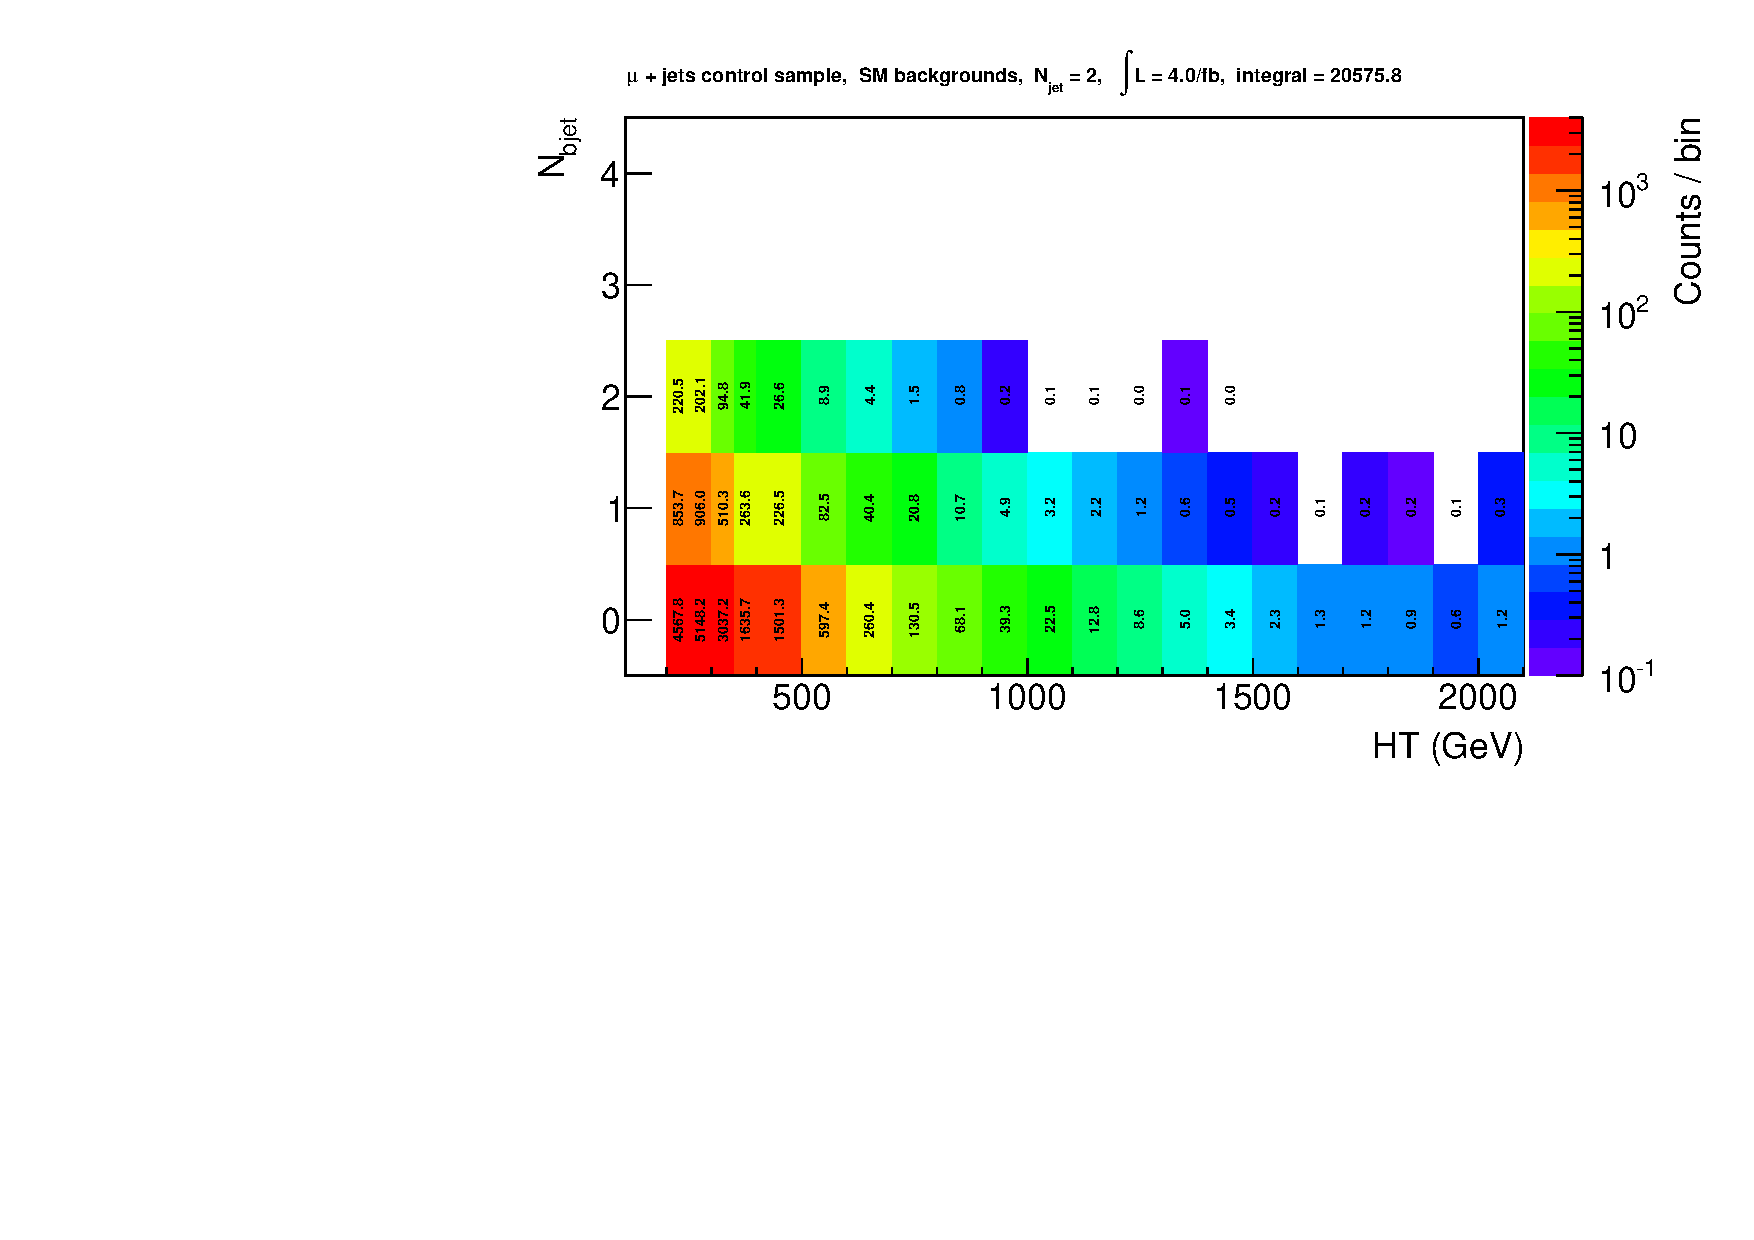
\includegraphics[width=0.5\textwidth]{figures/yieldPlots/mu_ewk_eq2j.pdf}
  }~~
  \subfigure[Yields from \texorpdfstring{\mj}{muon plus jets} control sample
  ($\njet = 3$)]{
    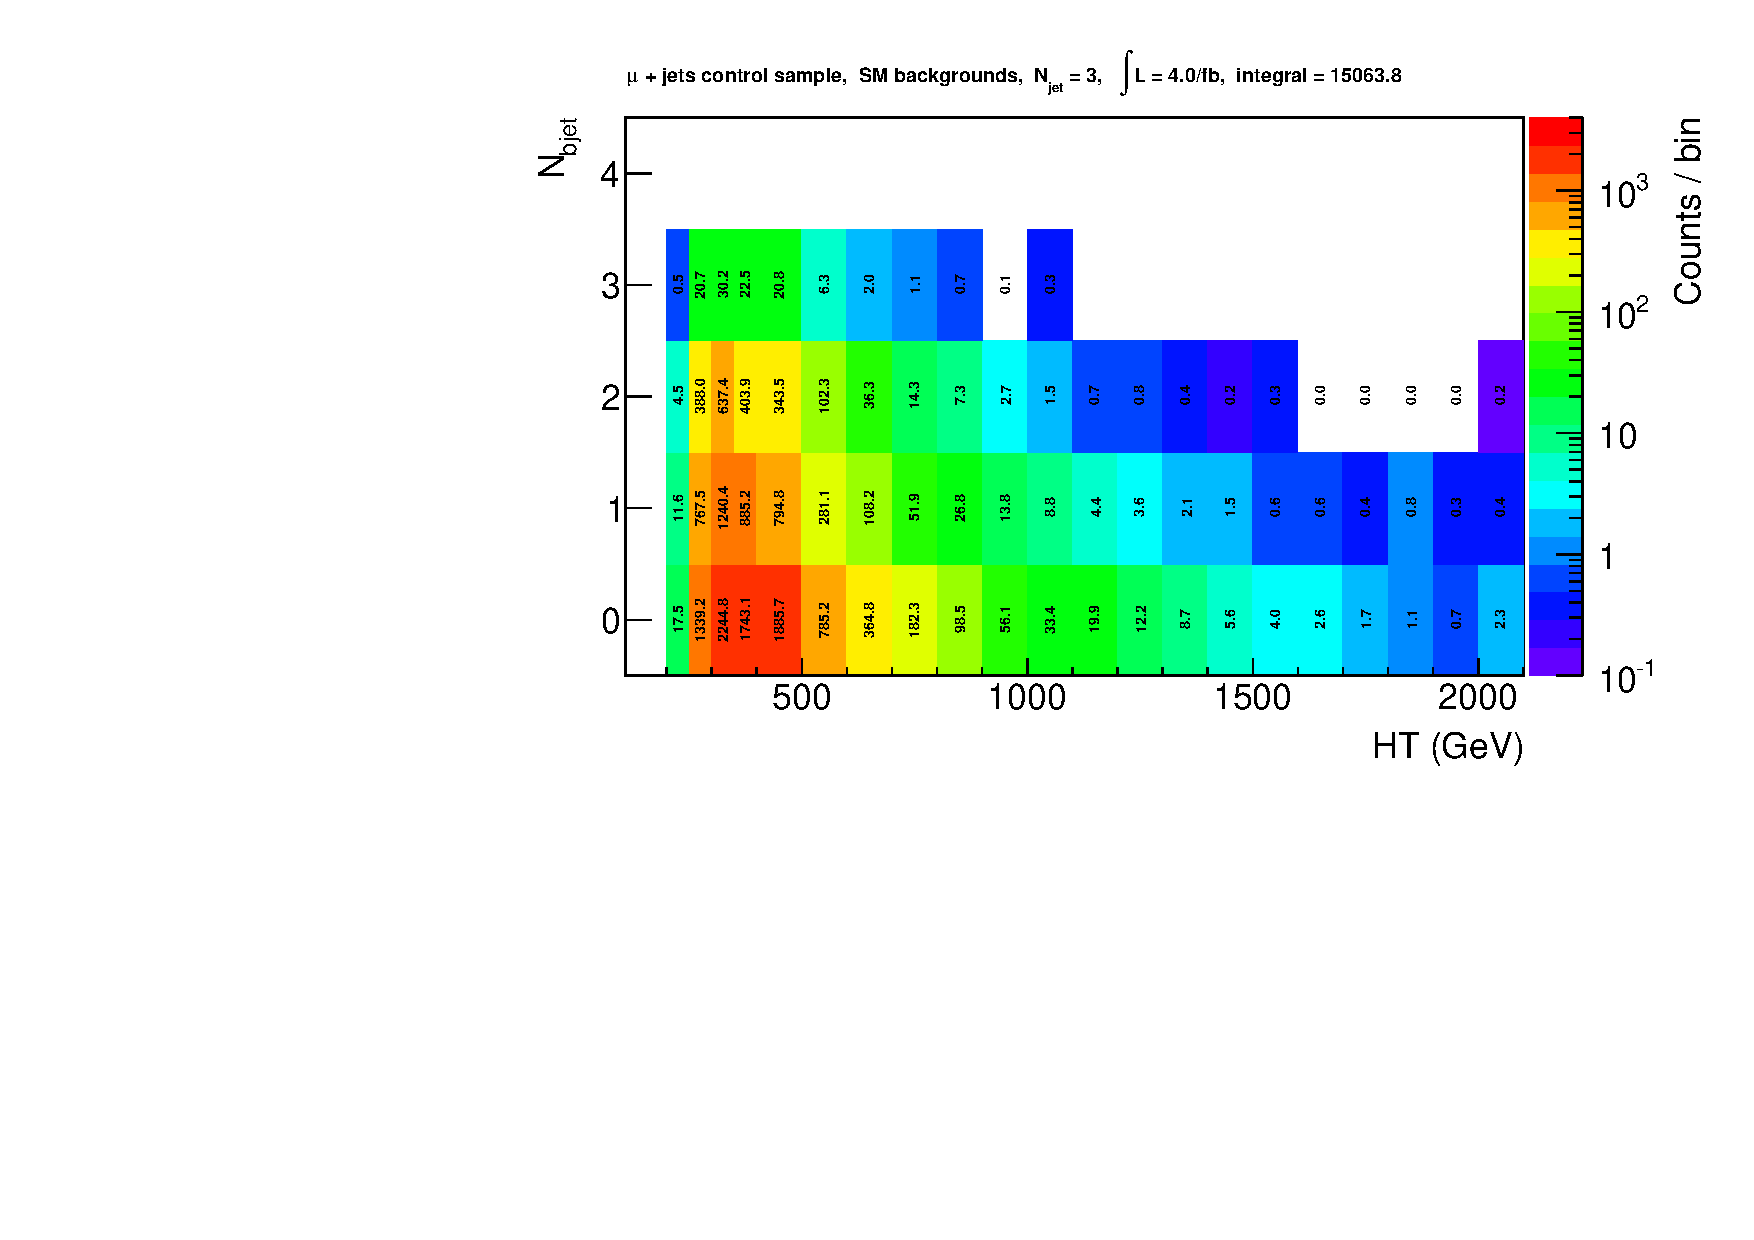
\includegraphics[width=0.5\textwidth]{figures/yieldPlots/mu_ewk_eq3j.pdf}
  }
  \\
  \subfigure[Yields from \texorpdfstring{\mj}{muon plus jets} control sample
  ($\njet = 4$)]{
    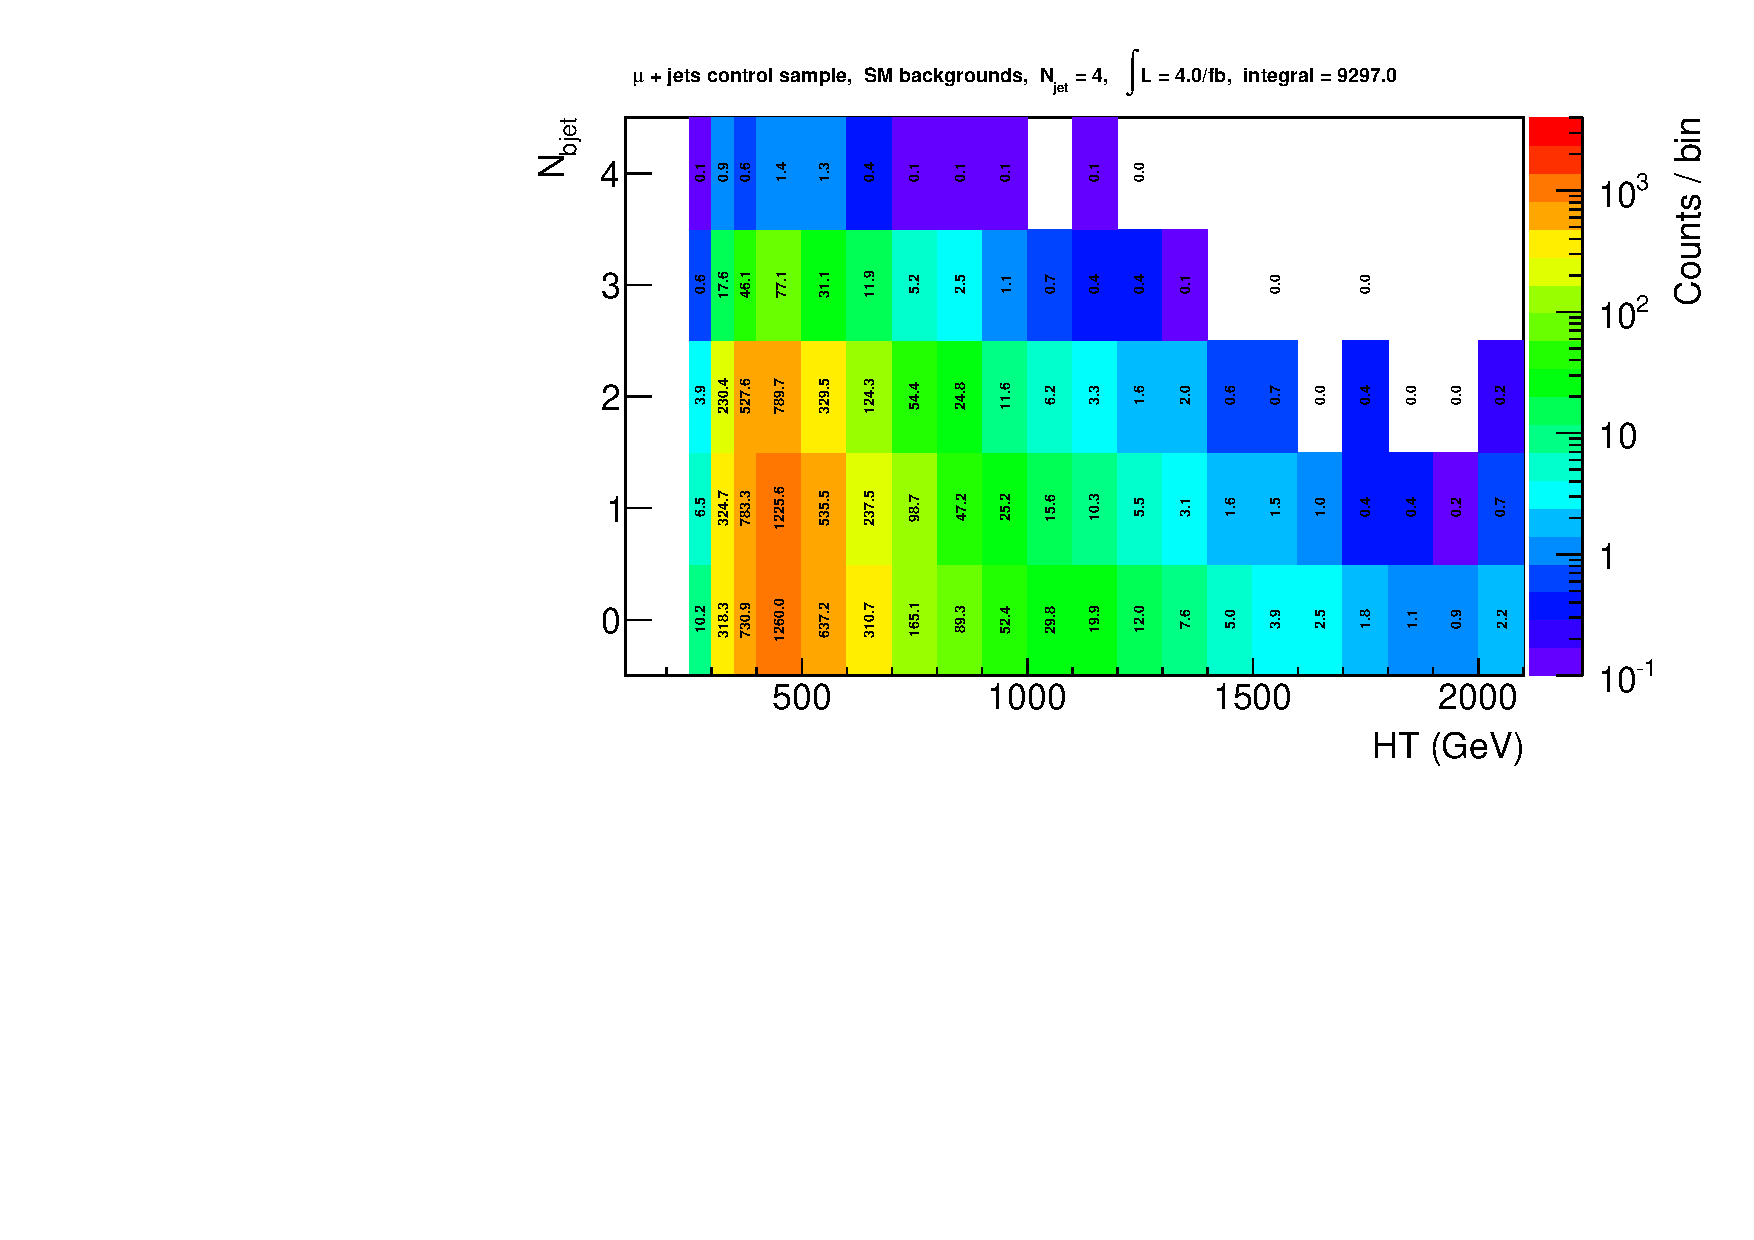
\includegraphics[width=0.5\textwidth]{figures/yieldPlots/mu_ewk_eq4j.pdf}
  }~~
  \subfigure[Yields from \texorpdfstring{\mj}{muon plus jets} control sample
  ($\njet \geq 5$)]{
    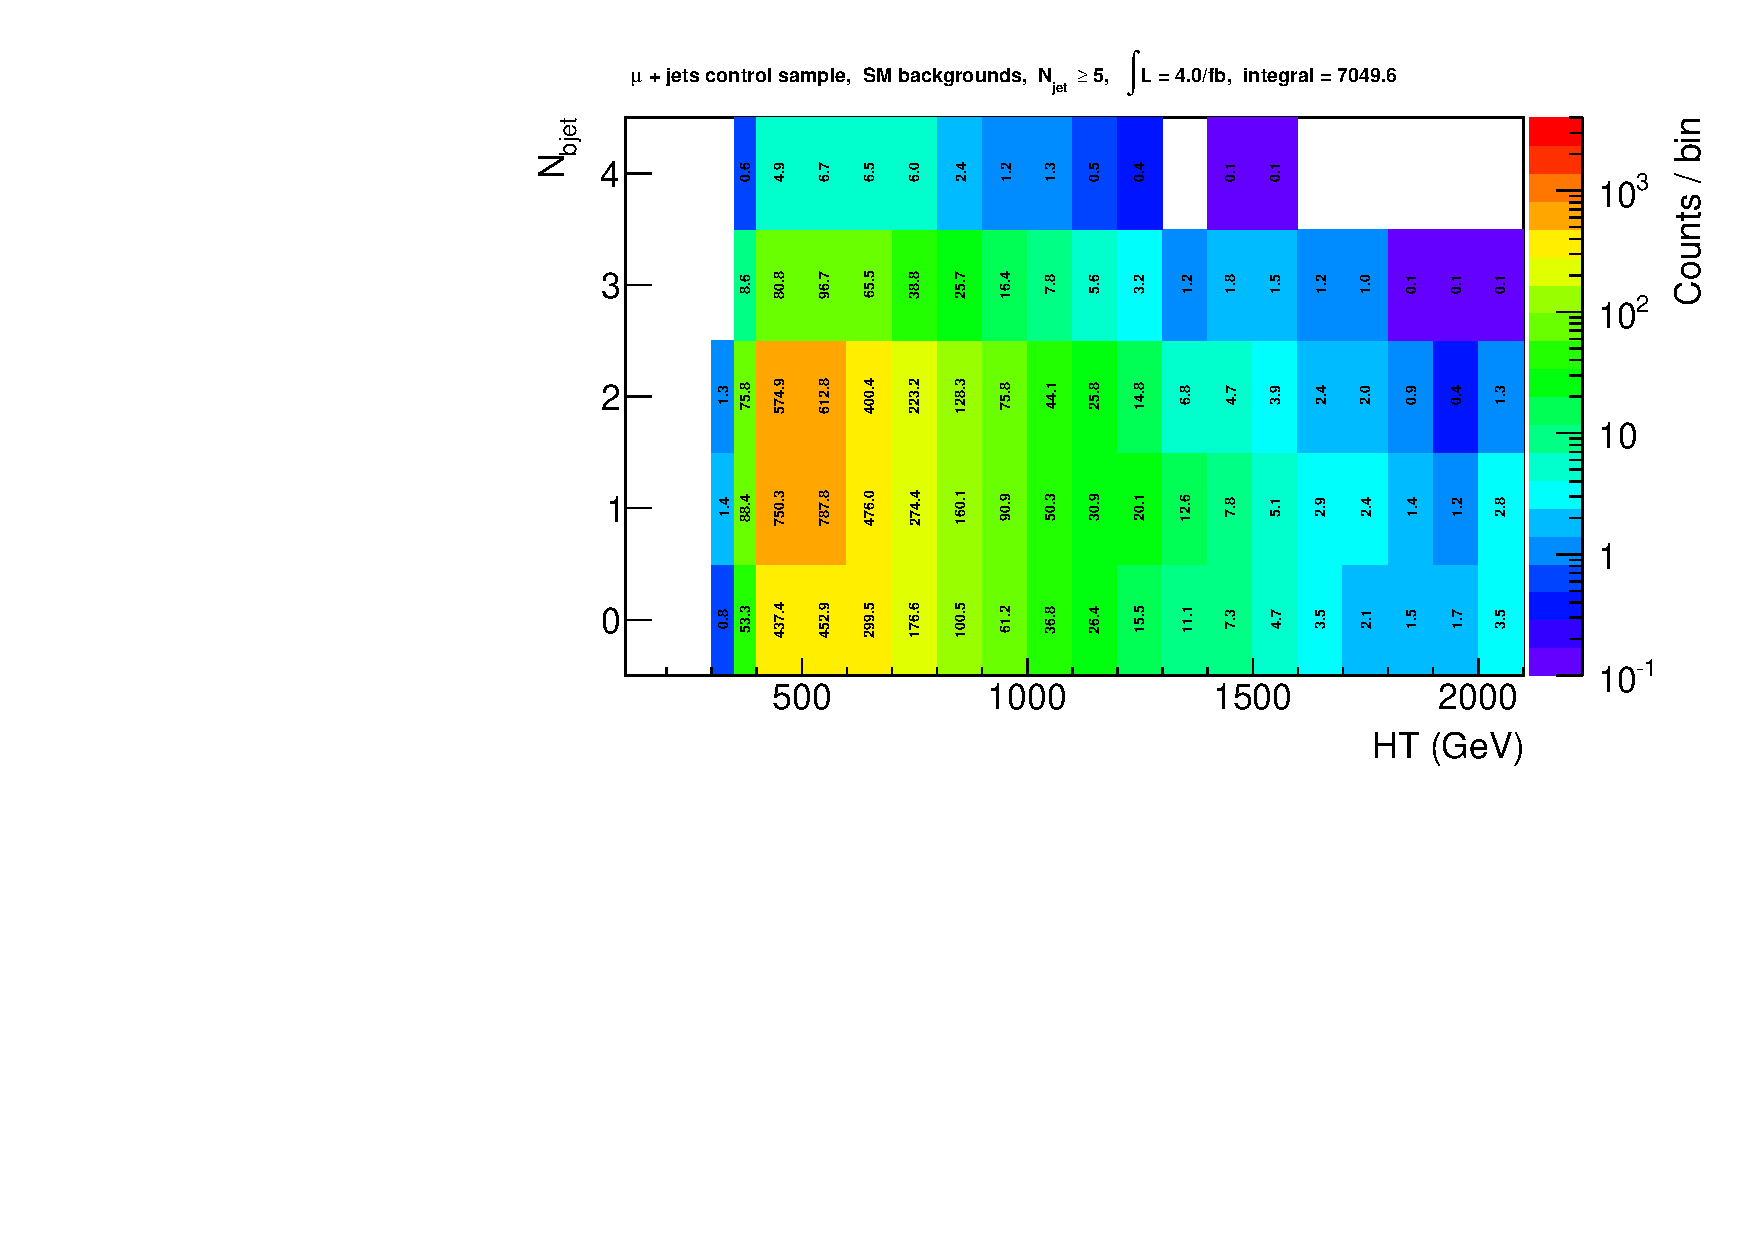
\includegraphics[width=0.5\textwidth]{figures/yieldPlots/mu_ewk_ge5j.pdf}
  } 
  \\
  \caption{\label{fig:muYields} Yields at $4\fbinv$ for the W~+~jets and \ttbar
  MC contributions to the \texorpdfstring{\mj}{muon plus jets} control sample. }
\end{figure}

\begin{figure}[h!]
  \centering
  \subfigure[Yields from \texorpdfstring{\mmj}{di-muon plus jets} control sample
  ($\njet = 2$)]{
    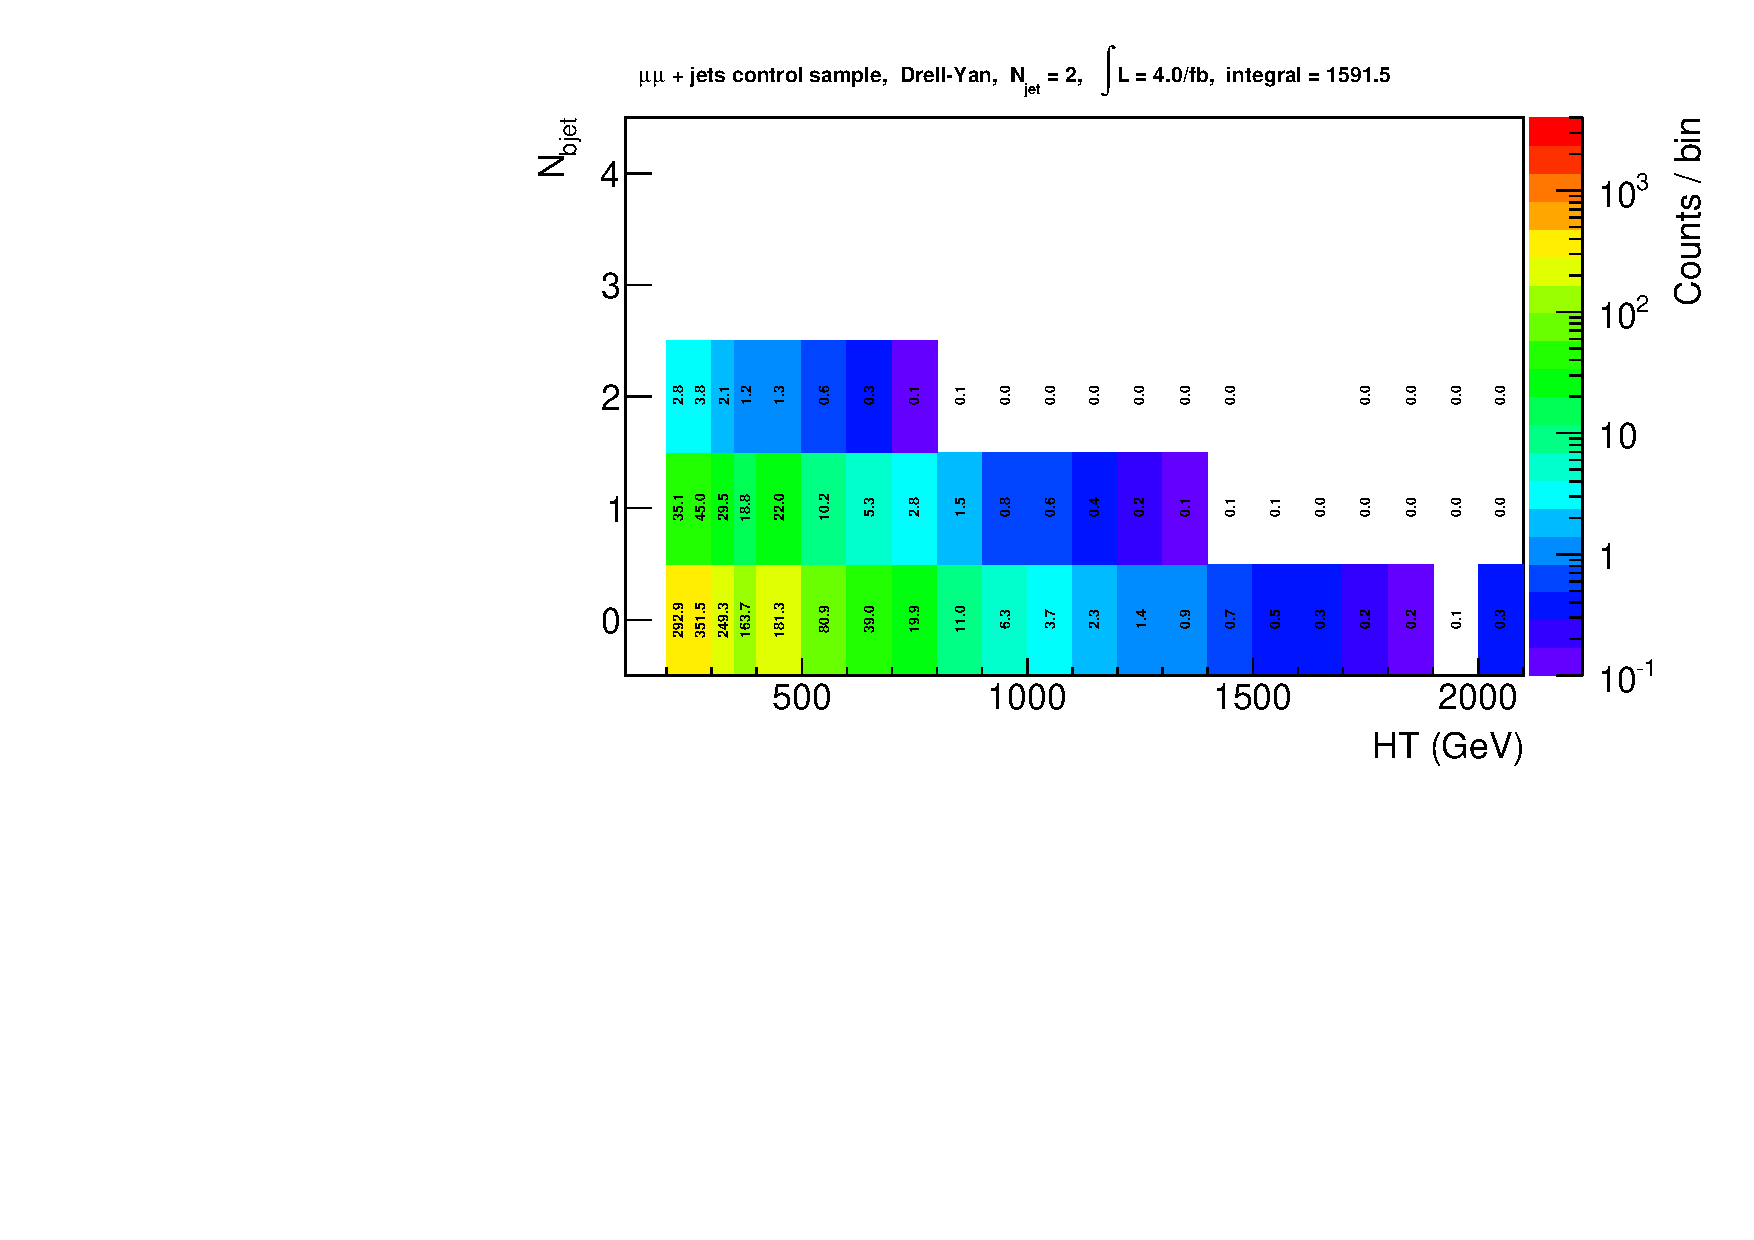
\includegraphics[width=0.5\textwidth]{figures/yieldPlots/mm_dy_eq2j.pdf}
  }~~
  \subfigure[Yields from \texorpdfstring{\mmj}{di-muon plus jets} control sample
  ($\njet = 3$)]{
    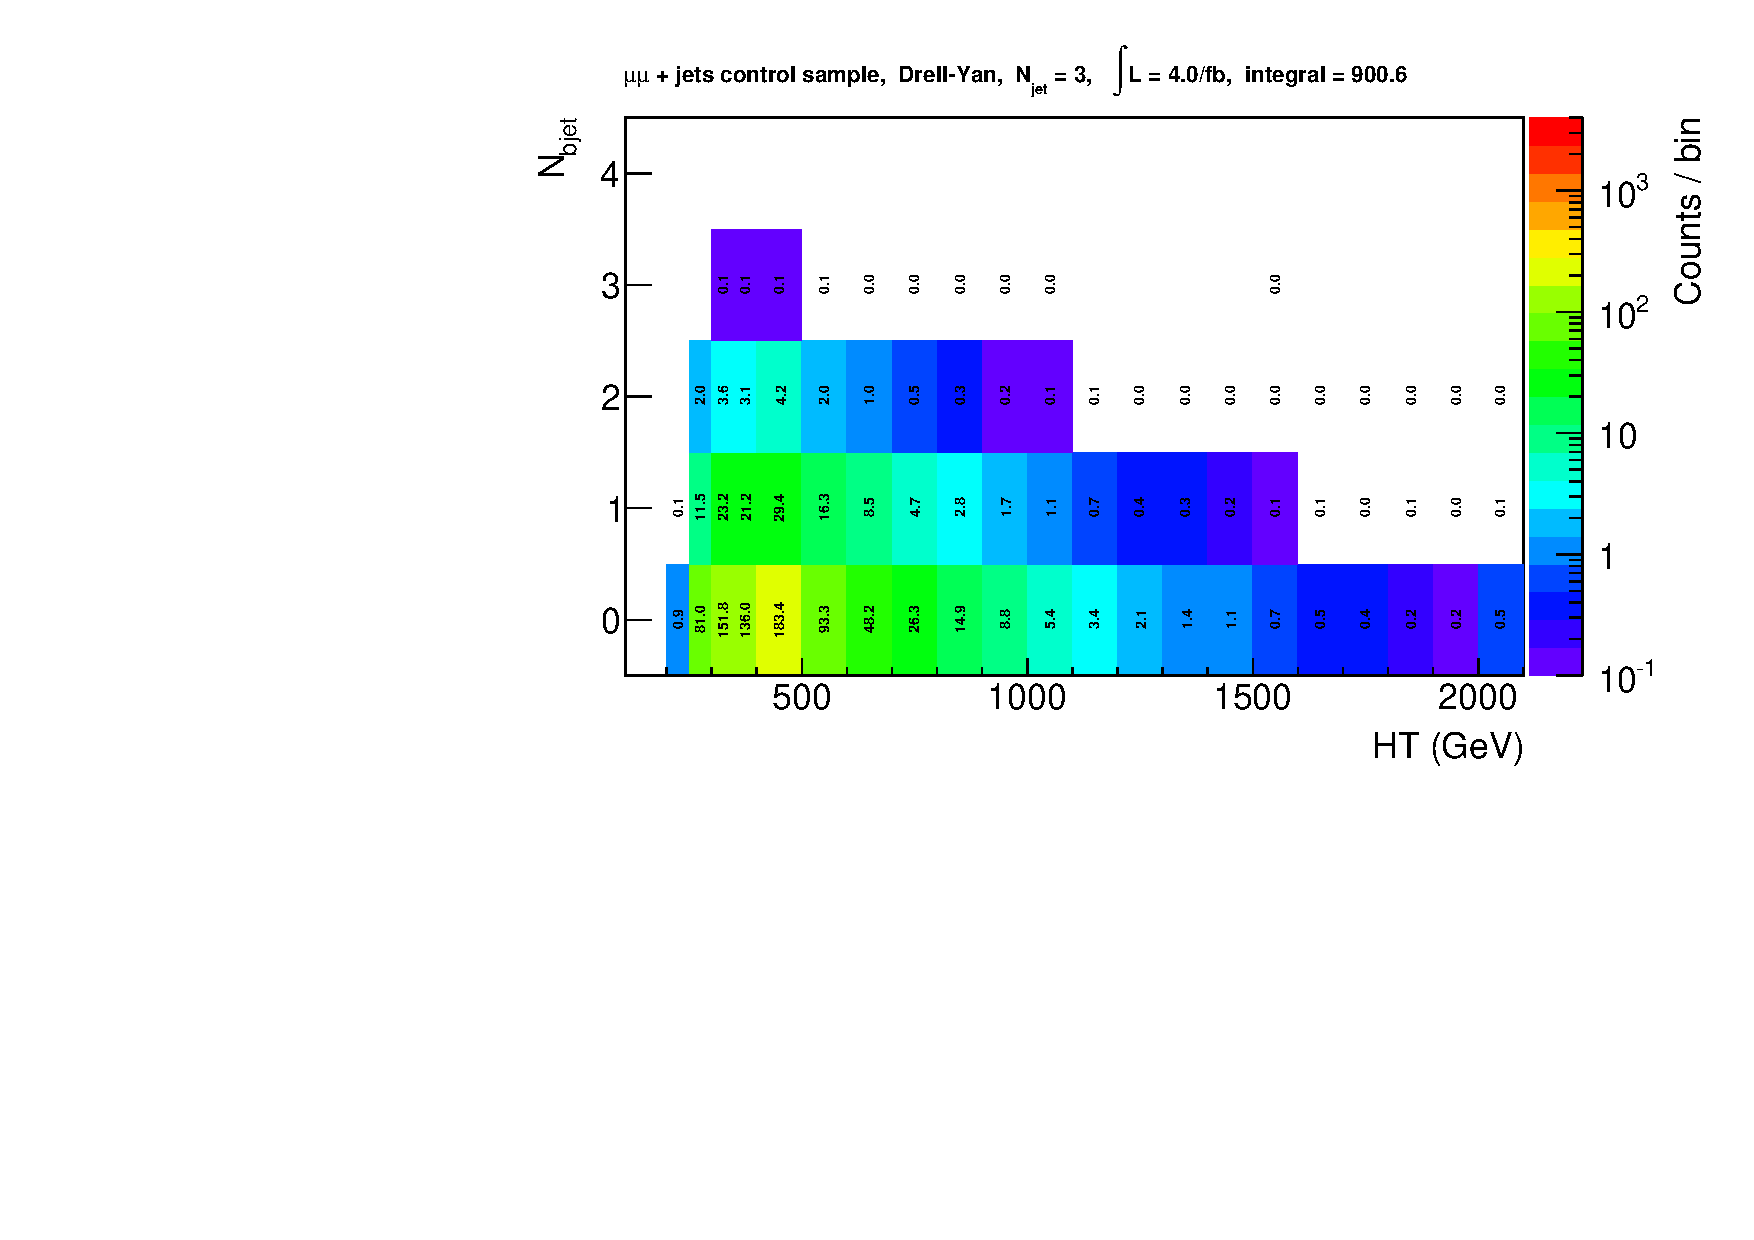
\includegraphics[width=0.5\textwidth]{figures/yieldPlots/mm_dy_eq3j.pdf}
  }
  \\
  \subfigure[Yields from \texorpdfstring{\mmj}{di-muon plus jets} control sample
  ($\njet = 4$)]{
    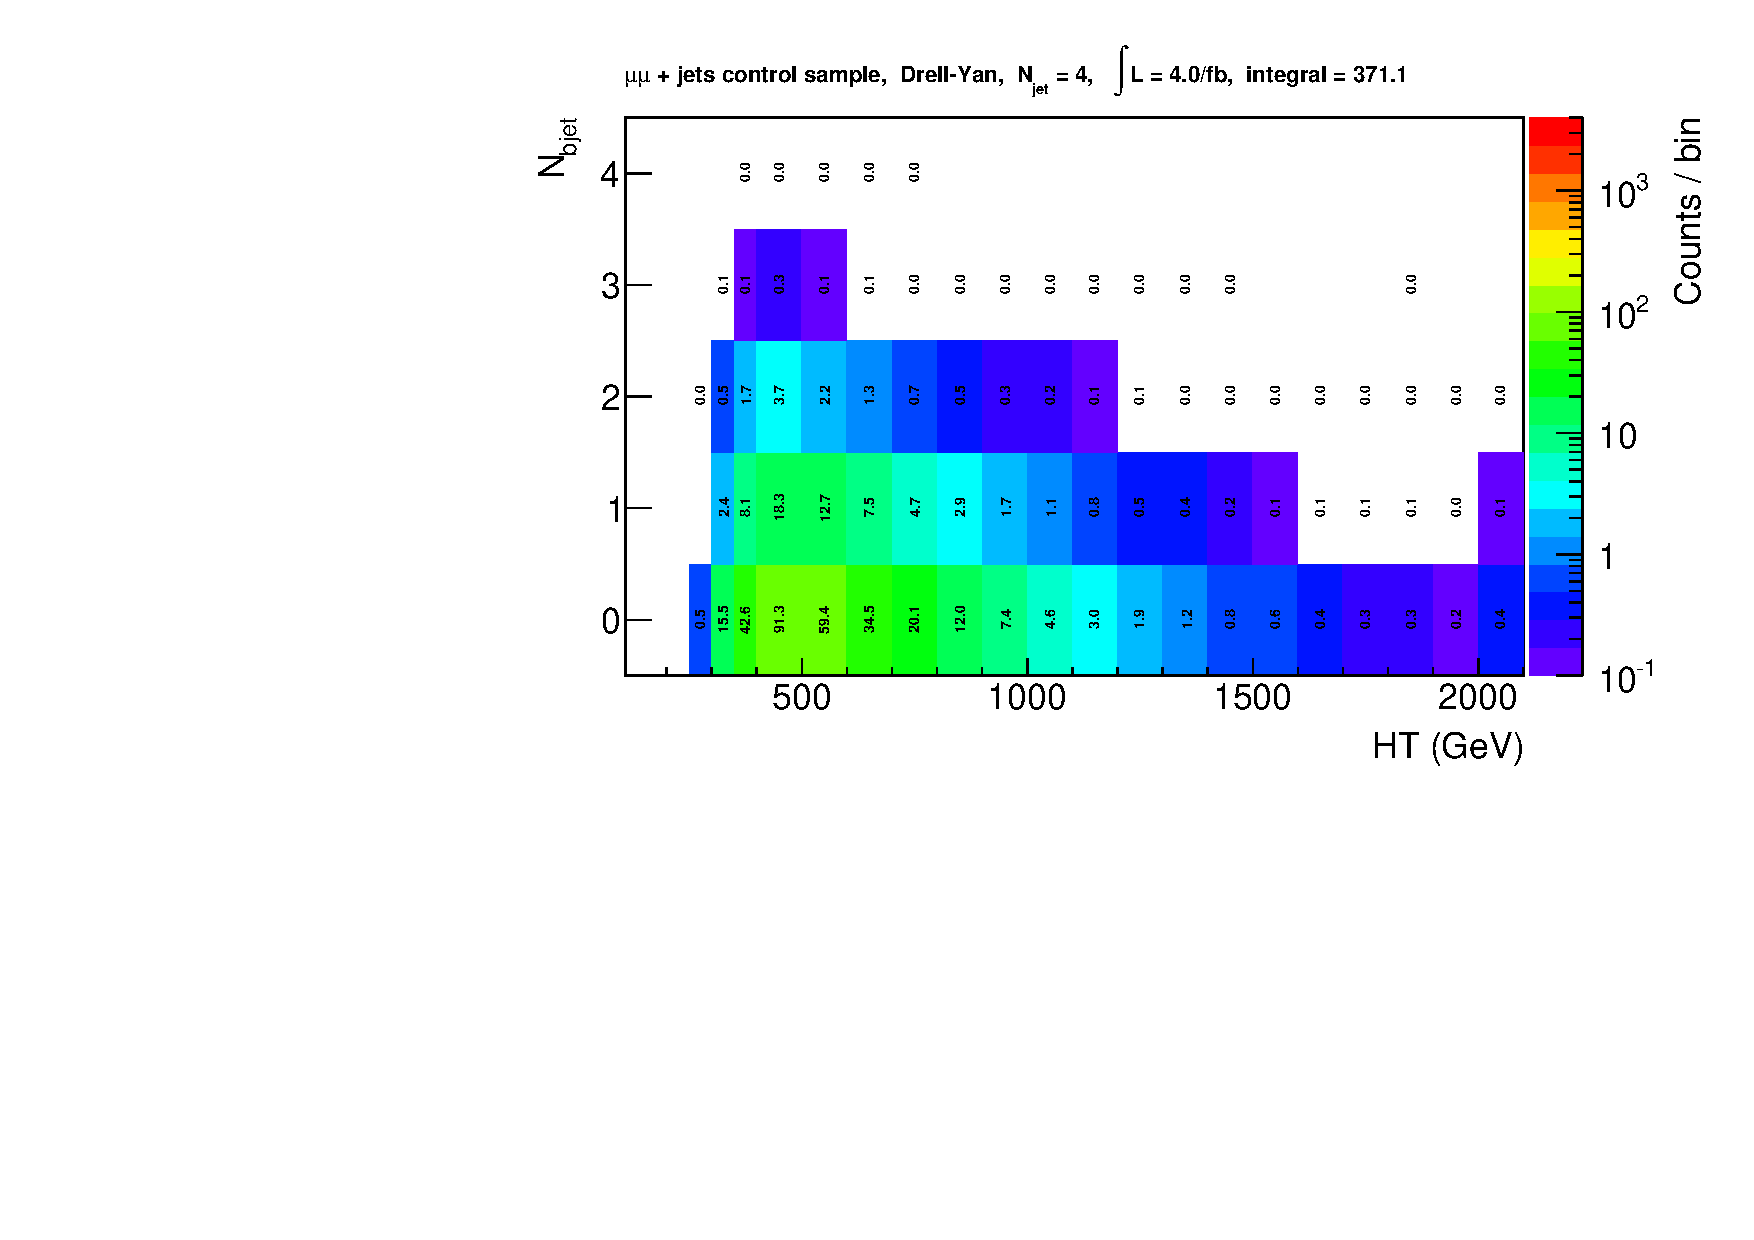
\includegraphics[width=0.5\textwidth]{figures/yieldPlots/mm_dy_eq4j.pdf}
  }~~
  \subfigure[Yields from \texorpdfstring{\mmj}{di-muon plus jets} control sample
  ($\njet \geq 5$)]{
    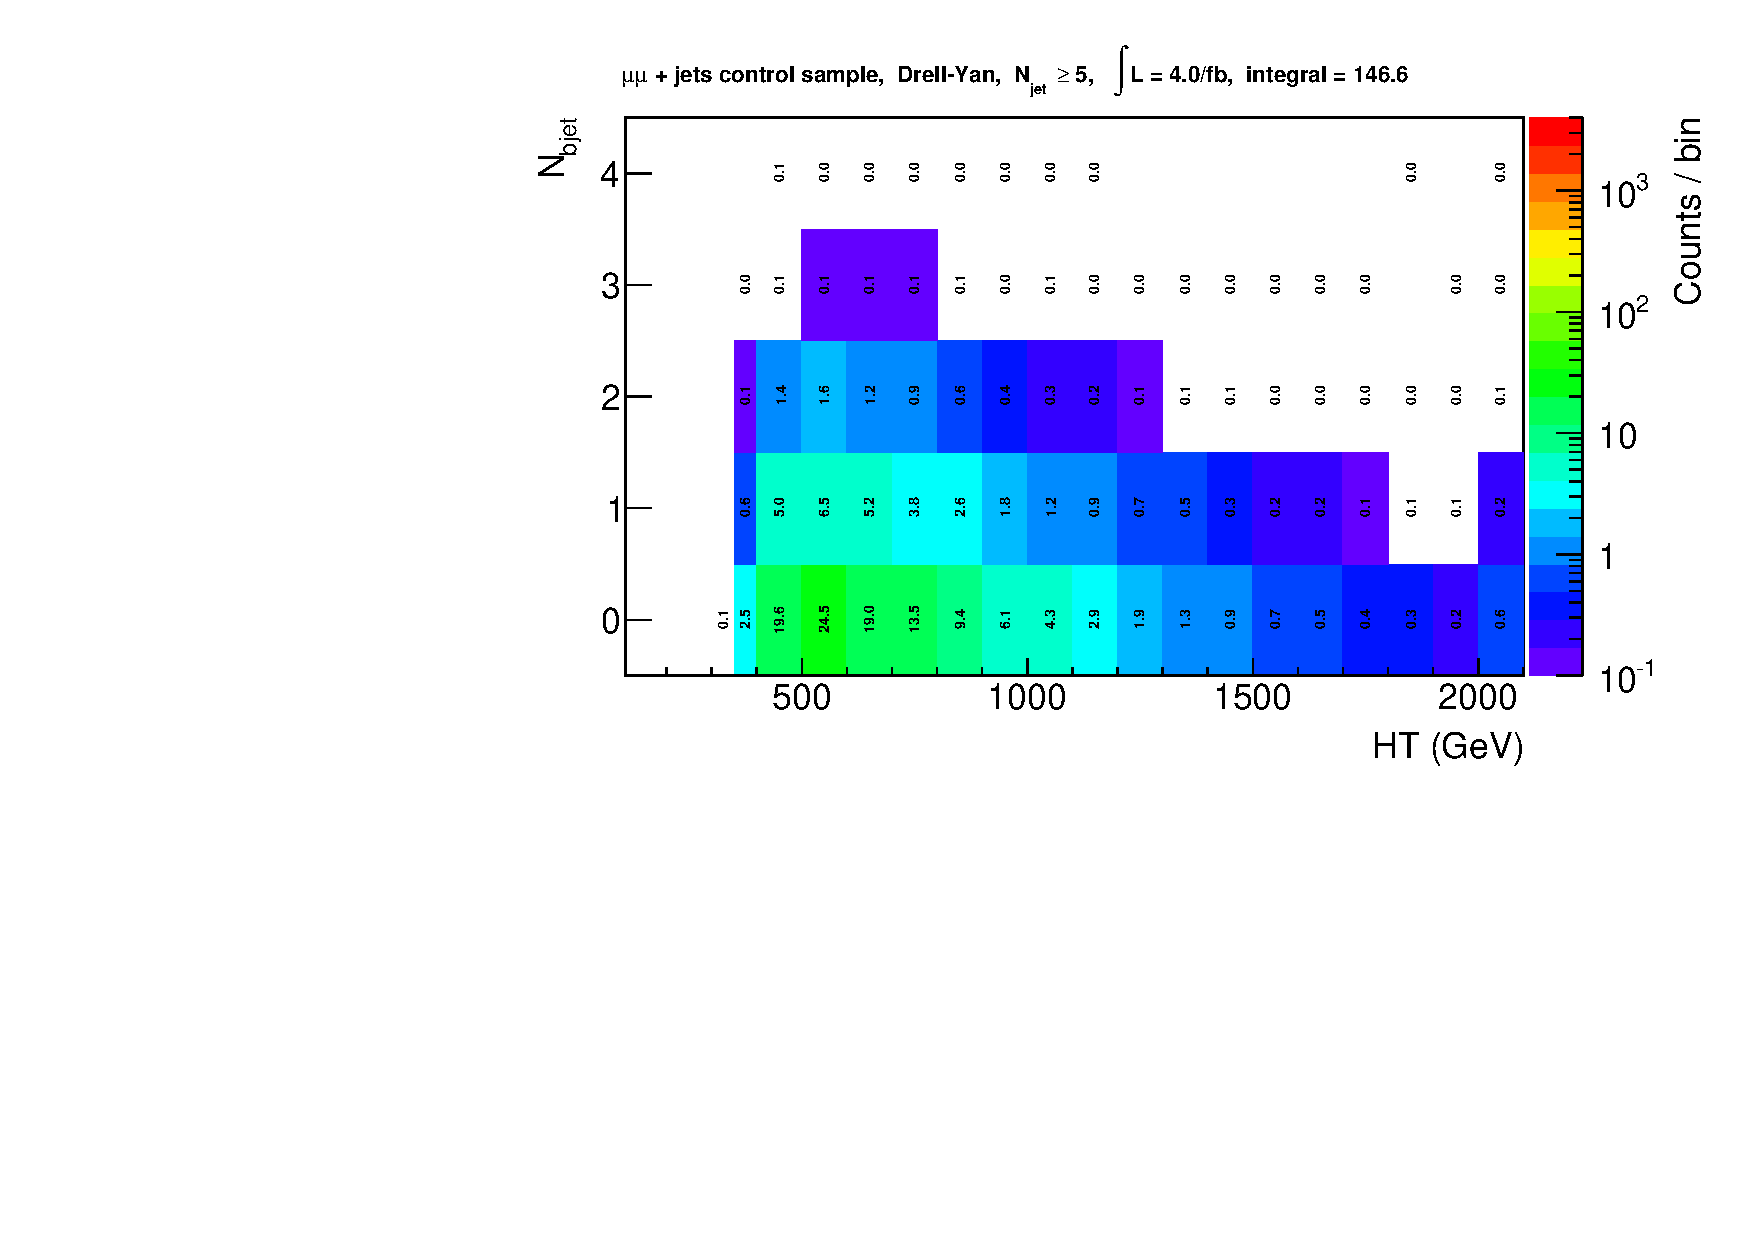
\includegraphics[width=0.5\textwidth]{figures/yieldPlots/mm_dy_ge5j.pdf}
  } 
  \\
  \caption{\label{fig:mumuYields} Yields at $4\fbinv$ for the DY~+~jets MC 
  contributions to the \texorpdfstring{\mmj}{di-muon plus jets} control sample. }
\end{figure}

\begin{figure}[h!]
  \centering
  \subfigure[Yields from \texorpdfstring{\gj}{photon plus jets} control sample
  ($\njet = 2$)]{
    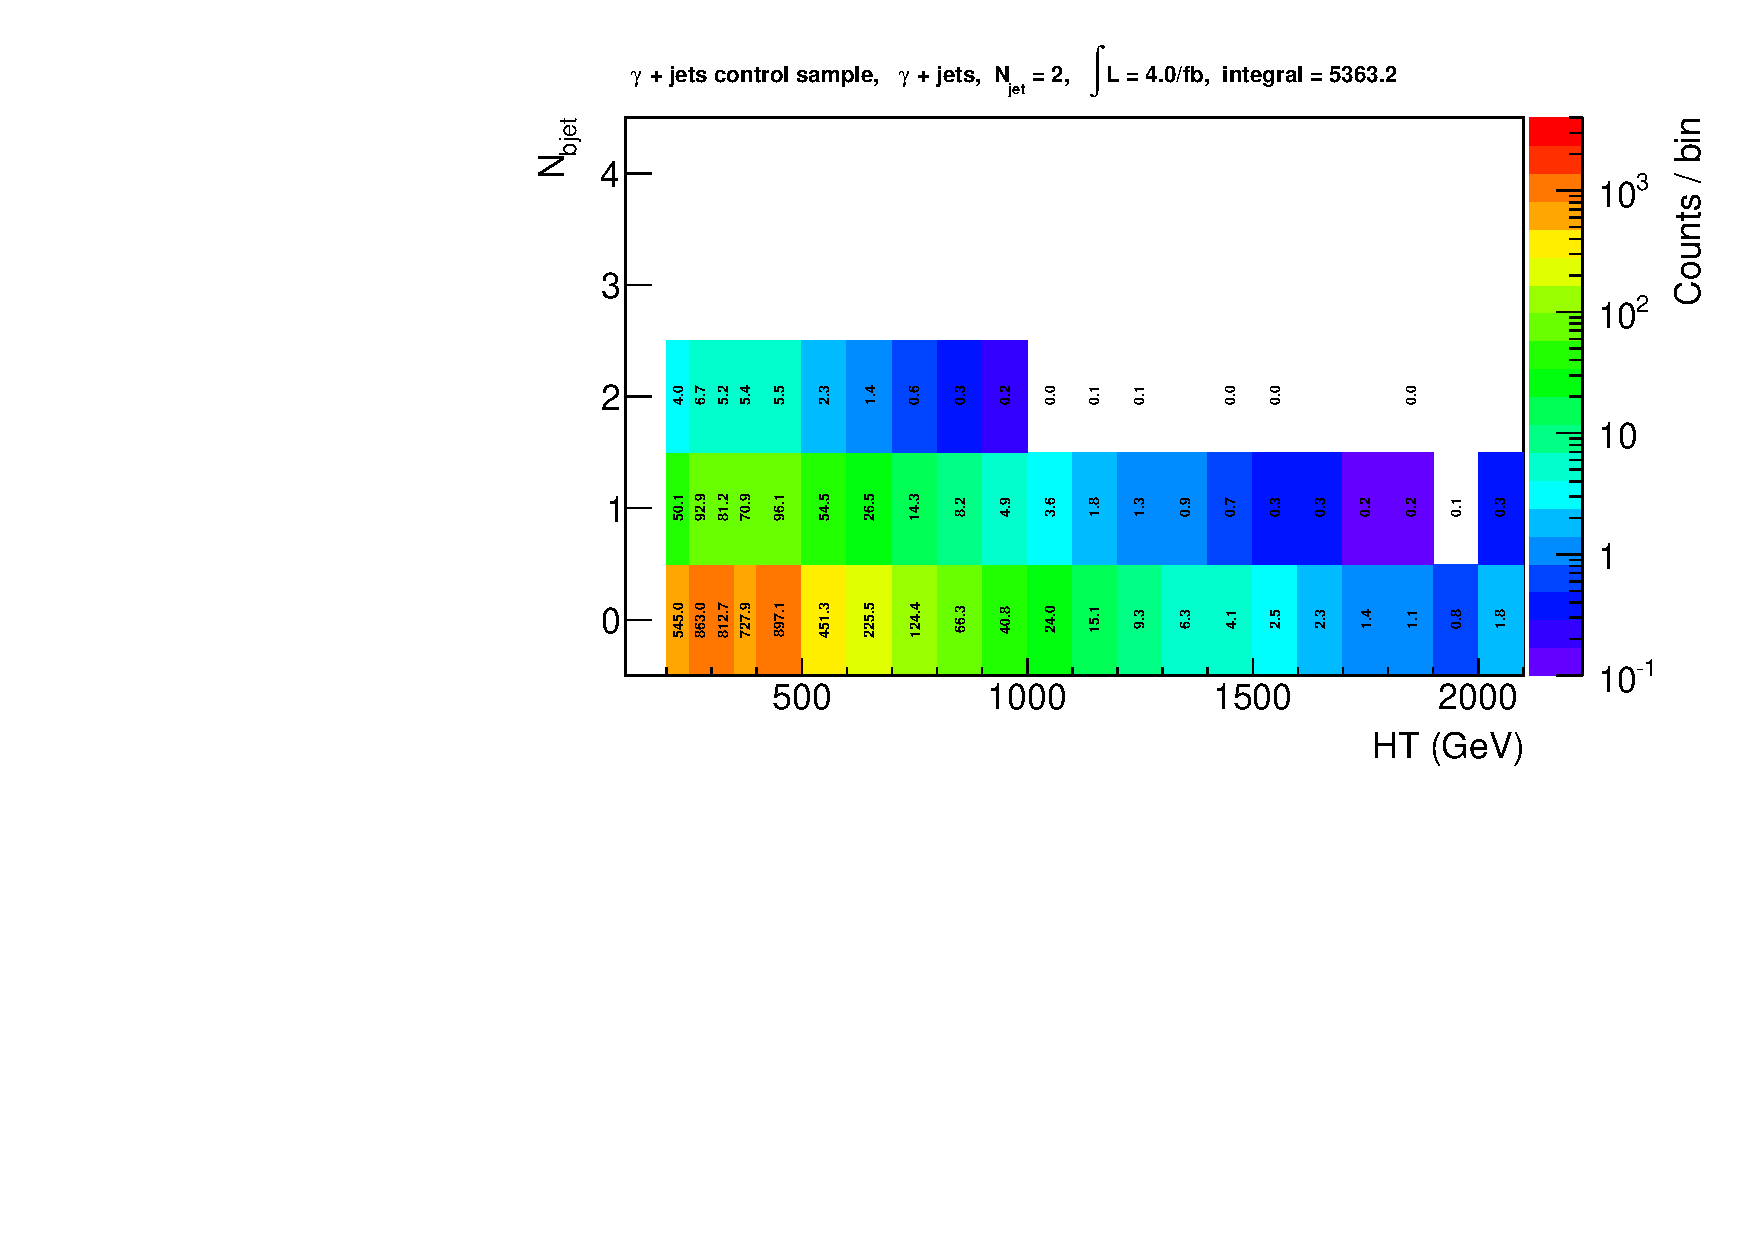
\includegraphics[width=0.5\textwidth]{figures/yieldPlots/ph_gjets_eq2j.pdf}
  }~~
  \subfigure[Yields from \texorpdfstring{\gj}{photon plus jets} control sample
  ($\njet = 3$)]{
    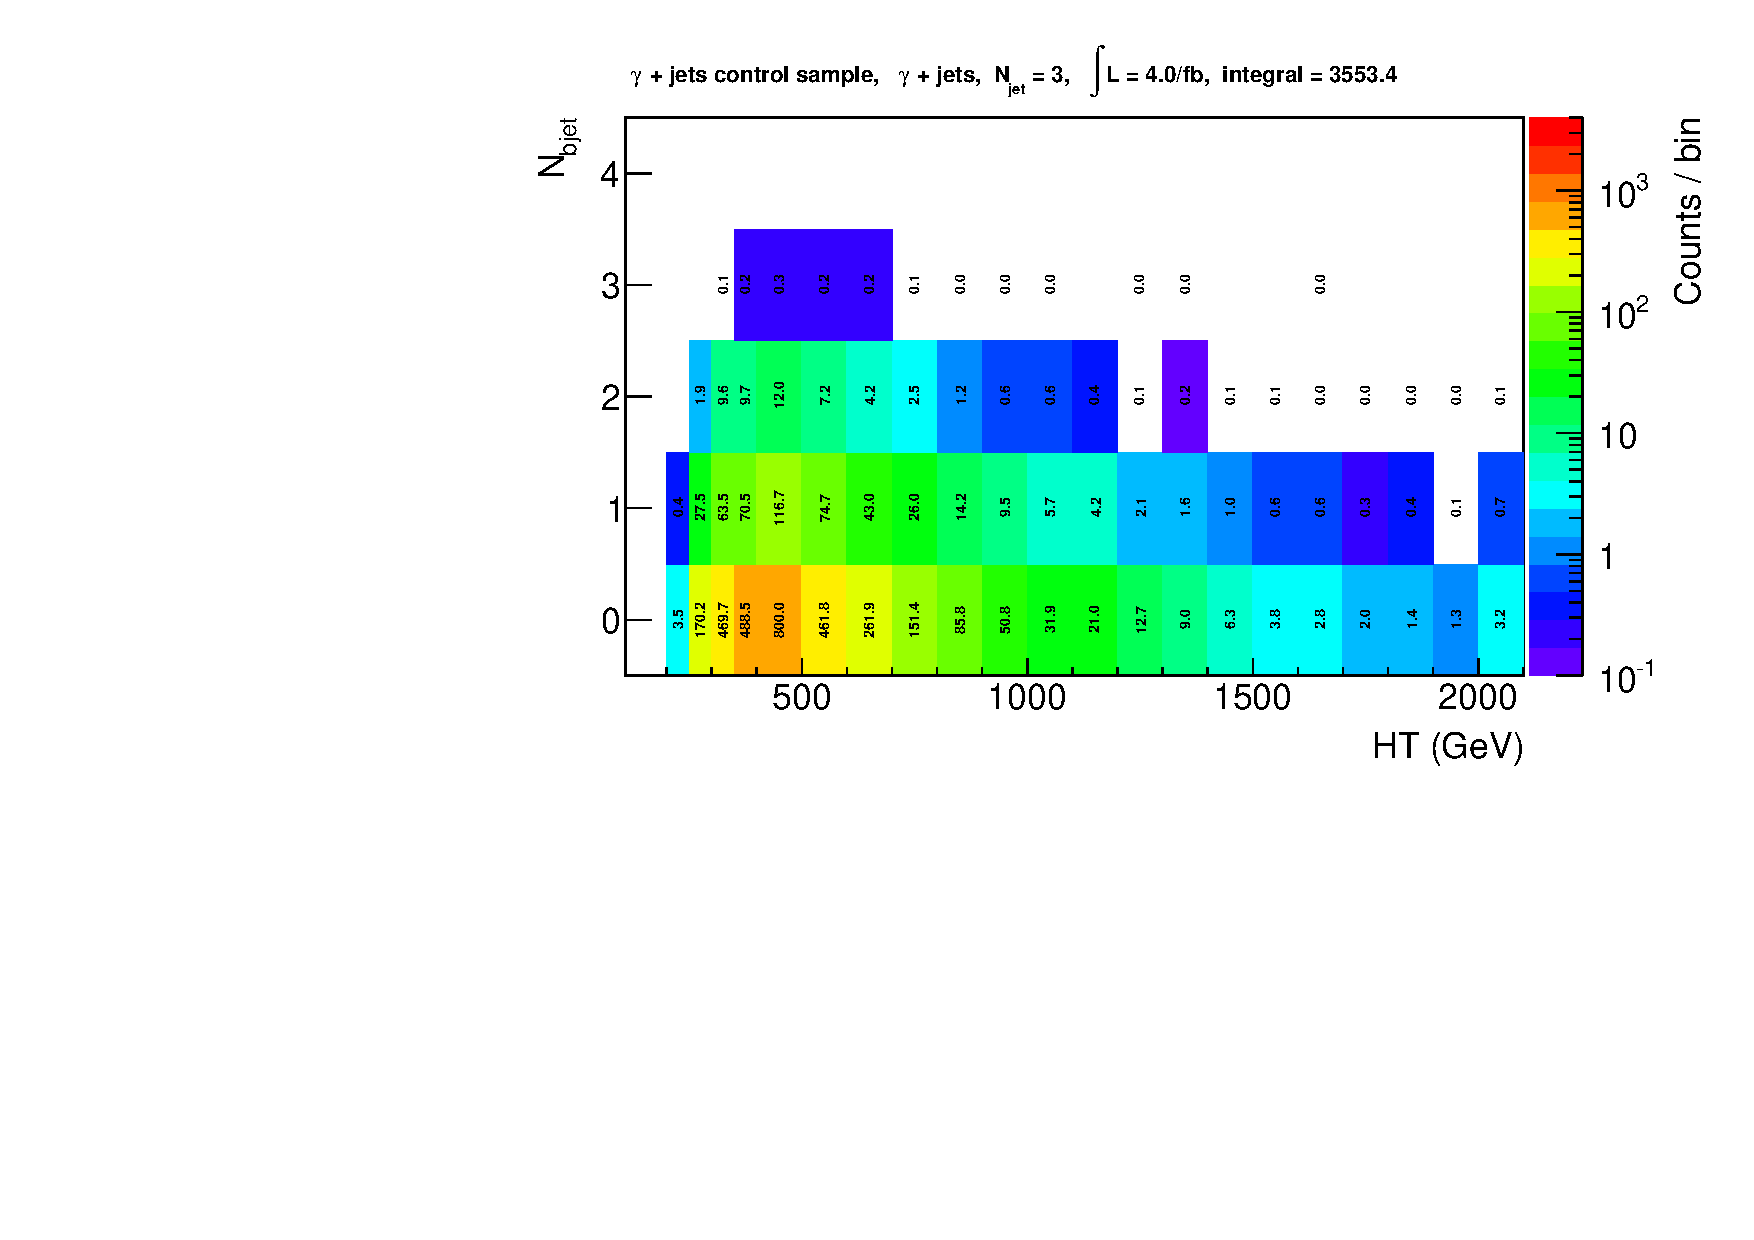
\includegraphics[width=0.5\textwidth]{figures/yieldPlots/ph_gjets_eq3j.pdf}
  }
  \\
  \subfigure[Yields from \texorpdfstring{\gj}{photon plus jets} control sample
  ($\njet = 4$)]{
    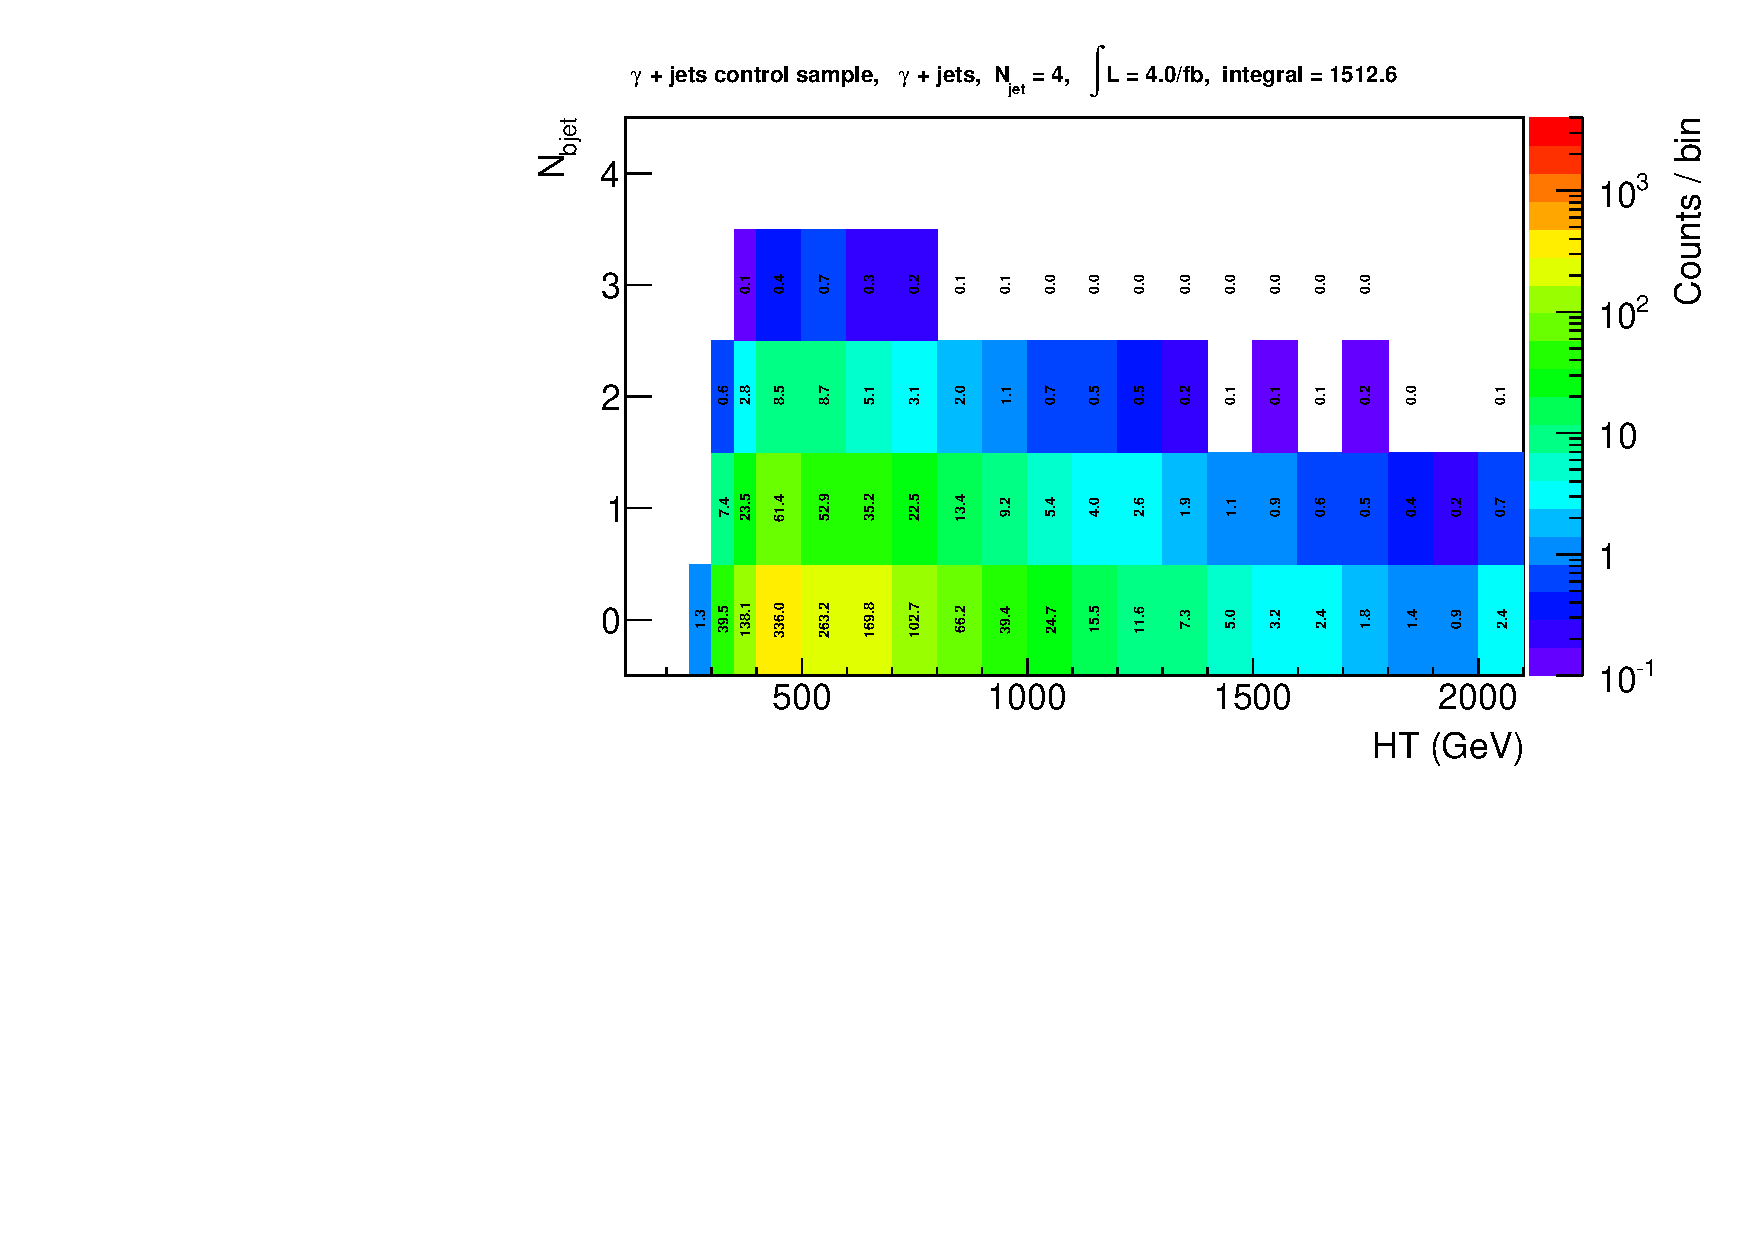
\includegraphics[width=0.5\textwidth]{figures/yieldPlots/ph_gjets_eq4j.pdf}
  }~~
  \subfigure[Yields from \texorpdfstring{\gj}{photon plus jets} control sample
  ($\njet \geq 5$)]{
    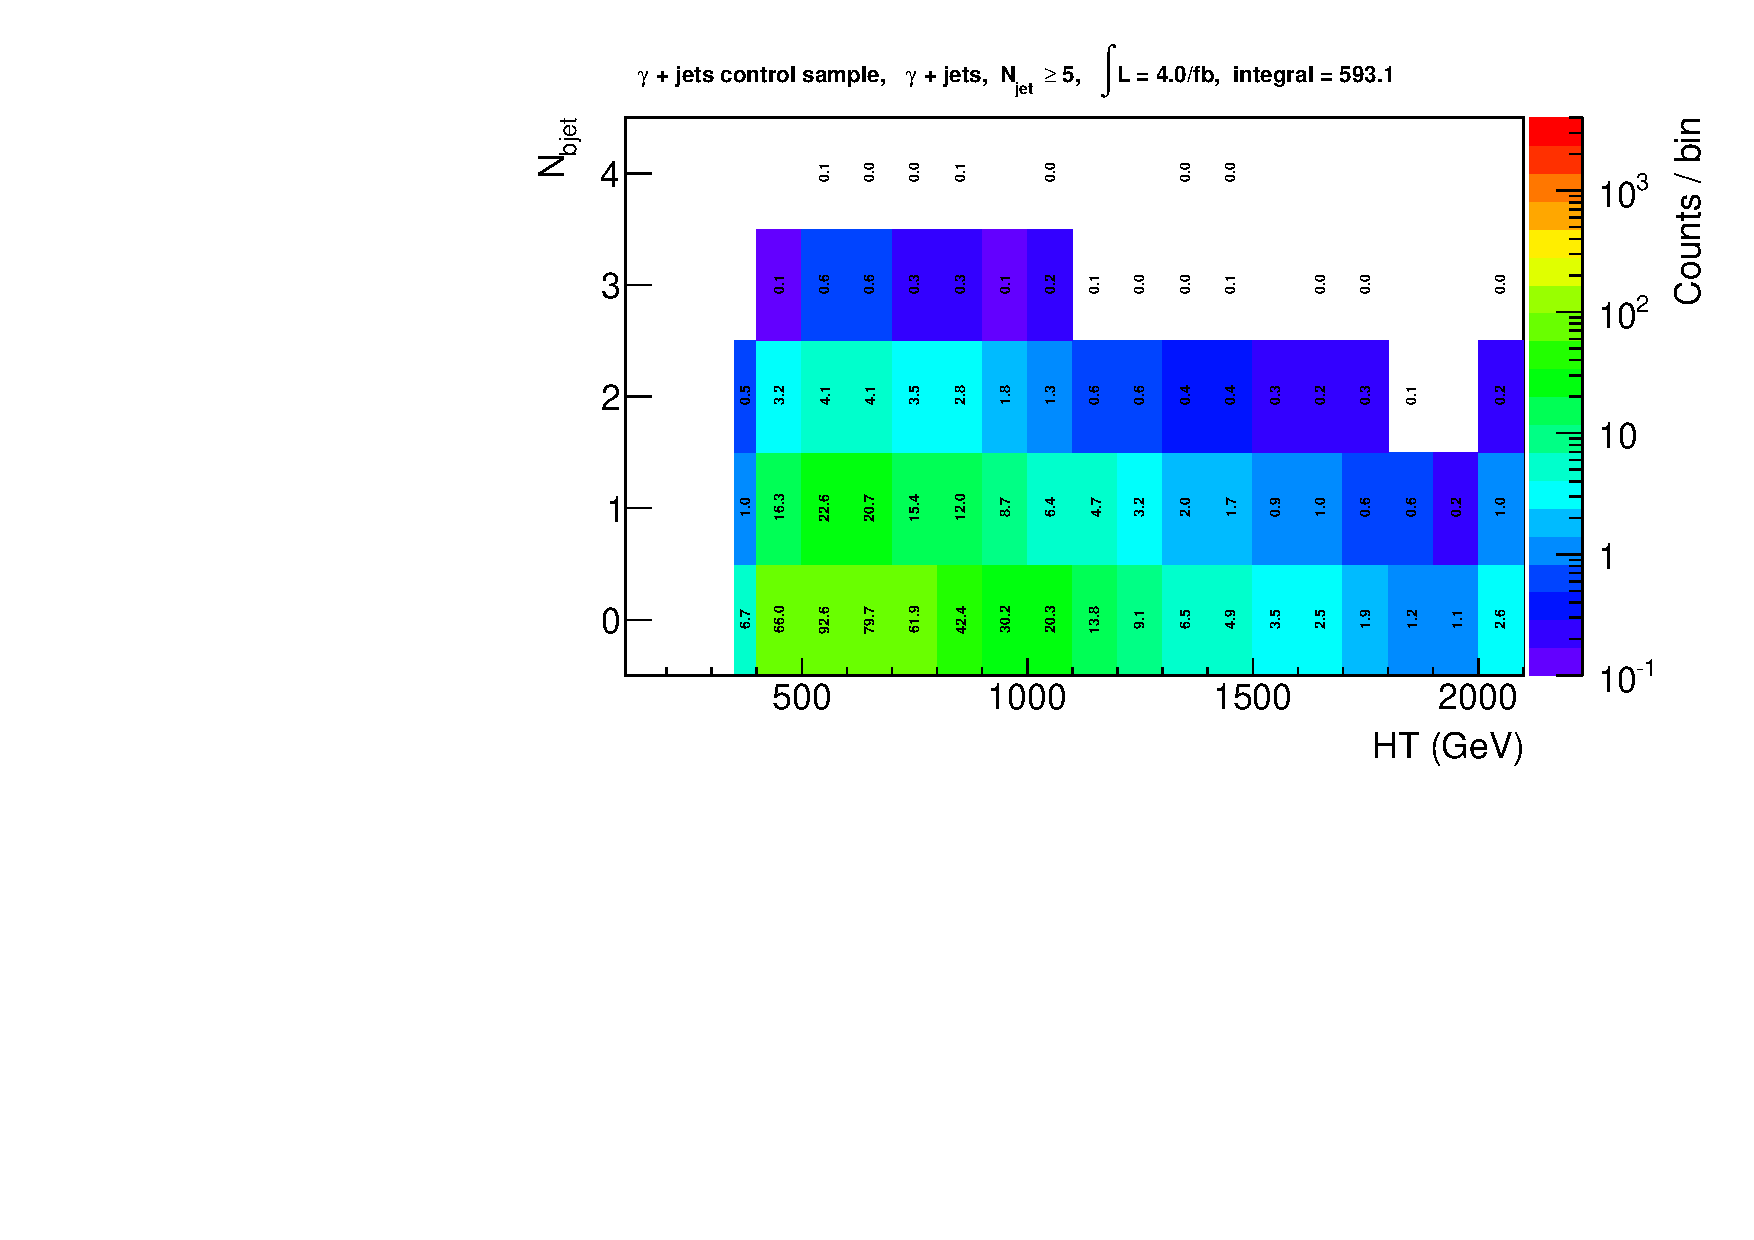
\includegraphics[width=0.5\textwidth]{figures/yieldPlots/ph_gjets_ge5j.pdf}
  } 
  \\
  \caption{\label{fig:gammaYields} Yields at $4\fbinv$ for the GJets MC 
  contributions to the \texorpdfstring{\gj}{photon plus jets} control sample. }
\end{figure}

%%____________________________________________________________________________||
\subsection{The improvement of sensitivity to SUSY models with binning changes}

\subsubsection{Gains from an asymmetric jet bin}

For a typical compressed model, Fig.~\ref{fig:asymMotivation} shows the second jet \PT
distribution for two different \HT bins. In the low \HT case a large portion of
the events are killed by requiring the second jet to have $\ET>100\gev$. 

It is therefore proposed to add an extra analysis category in which events with lead
jet $\ET>100\gev$ and second jet $40\gev<\ET<100\gev$. This new category will
result in new asymmetric jet bins split in $\njet$, $\nb$ and \HT. For the 
simplified model T2tt with $m_{stop}=425\gev$ and $m_{LSP}=325\gev$, 
including these bins increases signal acceptance by around a factor 3.

\begin{figure}[h!]
  \centering
  \subfigure[Second jet \PT for $200\gev<\HT<250\gev$, $\alphat>0.65$]{
    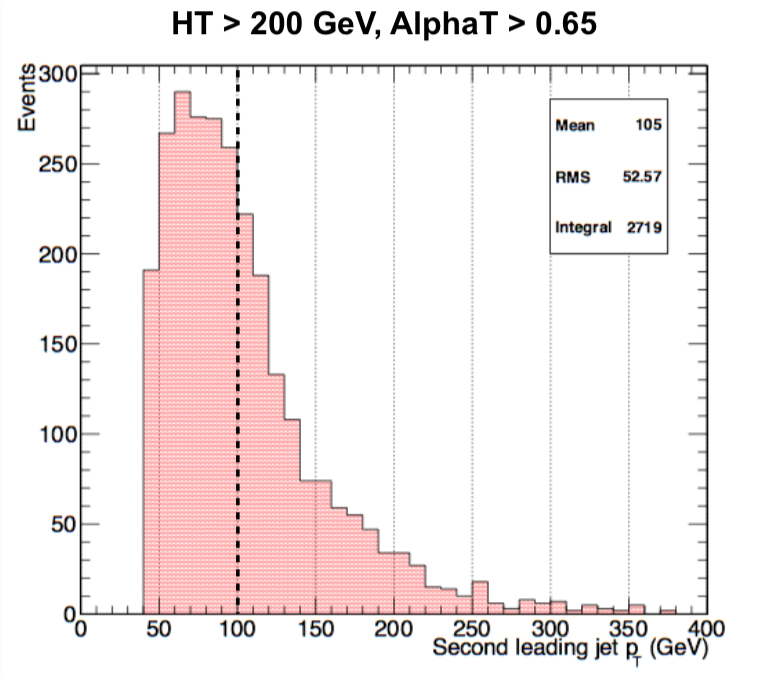
\includegraphics[width=0.5\textwidth]{figures/asymPlots/secondJetPtlowHT}
  }~~
  \subfigure[Second jet \PT for $400\gev<\HT>500\gev$, $\alphat>0.52$]{
    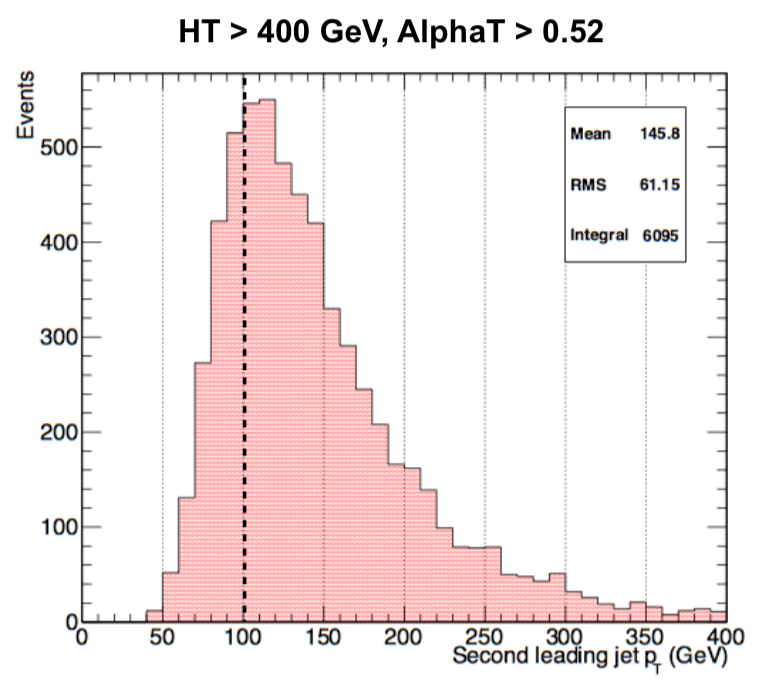
\includegraphics[width=0.5\textwidth]{figures/asymPlots/secondJetPthigherHT}
  }
  \\
  \caption{\label{fig:asymMotivation} The second leading jet \PT for different
  cases of \HT after a baseline signal selection: $\njet\geq2$, lead jet
  $\ET>100\gev$, lepton vetoes. Made using the XXX sample.}
\end{figure}

NOTE: which sample did the second jet pt plots come from?

\subsubsection{Extension of \HT bins}

The production of heavy SUSY particles, such as gluino pair
production, will result in large values of \HT . This is illustrated in the high 
\HT of events in Fig.~\ref{fig:sigYields}. To increase the sensitivity
of the analysis to these kinds of models, the \HT bins can be extended to higher
values. The only limit placed on this value is that there are enough events in the
relevant control samples, to allow a data driven background prediction. The
number of events is deemed to be sufficient when their statistical uncertainty is
approximately equal to the expected systematic uncertainty for the bin in
question. Initial studies suggest it should be possible to extend up to
$\HT=1600$, possibly even $\HT=2000$. This would give a great increase in the
signal over background ratio, particularly for gluino mediated models.

%%____________________________________________________________________________||
\subsection{The improvement of sensitivity to dark matter models with improved binning }

PLACEHOLDER: DM yield table here or in Bjoern's section?
%%____________________________________________________________________________||
